\documentclass[11pt]{article} % use larger type; default would be 10pt

\usepackage[utf8]{inputenc} % set input encoding (not needed with XeLaTeX)
\usepackage{amsmath,amssymb}
\usepackage{bm}
\usepackage{natbib}
\usepackage{hyperref}
\usepackage{graphicx}
\usepackage{mathtools}
\usepackage{fullpage}
\usepackage{makecell}
\usepackage{booktabs}
\usepackage{multirow}
\usepackage{../../../generalCode/numdef}

\newcommand{\reg}[2]{g\left(#1;#2\right)}
\newcommand{\regc}[2]{g_C\left(#1;#2\right)}
\newcommand{\regt}[2]{g_T\left(#1;#2\right)}
\newcommand{\bx}{\bm{x}}
\newcommand{\bxi}{\bm{x}_i}
\newcommand{\bxs}{\bx}%{\bx^S}
\newcommand{\bxy}{\bx^Y}
\newcommand{\bxyt}{\bx^{Y\prime}}
\newcommand{\bxsi}{\bxs_i}
\newcommand{\bxsit}{\bm{\tilde{x}^S}_i}
\newcommand{\bxsitp}{\bm{\tilde{x}^{S\prime}}_i}
\newcommand{\EE}{\mathbb{E}}
\newcommand{\pp}{e(\bxs)}
\newcommand{\ppi}{e(\bxsi)}
\newcommand{\ppip}[1]{e_{#1}(\bxsi)}
\newcommand{\hpp}{\hat{e}(\bxs)}
\newcommand{\hppi}{\hat{e}(\bxsi)}
\newcommand{\ppf}[2]{e_{#1}\left(#2\right)}
\newcommand{\yt}{Y_T}
\newcommand{\yc}{Y_C}
\newcommand{\yti}{Y_{Ti}}
\newcommand{\yci}{Y_{Ci}}
\newcommand{\sti}{S_{Ti}}
\newcommand{\sci}{S_{Ci}}
\newcommand{\st}{S_T}
\num\newcommand{\eff0}{\tau^0}
\num\newcommand{\eff1}{\tau^1}
\num\newcommand{\mut1}{\mu_T^1}
\num\newcommand{\mut0}{\mu_T^0}
\num\newcommand{\muc1}{\mu_C^1}
\num\newcommand{\muc0}{\mu_C^0}
\num\newcommand{\heff0}{\hat{\tau}^0}
\num\newcommand{\heff1}{\hat{\tau}^1}
\newcommand{\mucs}{\mu_C^s}
\newcommand{\muts}{\mu_T^s}
\newcommand{\effs}{\tau^s}
\newcommand{\ri}{R_i}
\newcommand{\blam}{\bm{\Lambda}}
\newcommand{\dblam}{\bm{\dot{\Lambda}}}
\newcommand{\blamh}{\bm{\hat{\Lambda}}}
%\newcommand{\r}{R}


\newcommand\independent{\protect\mathpalette{\protect\independenT}{\perp}}
\def\independenT#1#2{\mathrel{\rlap{$#1#2$}\mkern2mu{#1#2}}}


\theoremstyle{plain}
\newtheorem{prop}{Proposition}
\newtheorem{lemma}{Lemma}

\theoremstyle{remark}
 \newtheorem{ass}{Assumption}


\title{GEEPERS: Principal Stratification using Principal Scores and Stacked Estimating Equations}

\begin{document}
\maketitle

\section{Introduction}

Randomized experiments easily admit subgroup analysis---estimation of treatment effects for a subset of the study population---when those subgroups are defined at baseline, and not themselves a function of treatment assignment.
A simple, popular approach to estimating subgroup effects is to use ordinary least squares (OLS) regression, regressing the outcome on a treatment indicator interacted with an indicator for subgroup membership.
However, when subgroup membership is a function of a post-treatment variable, then it may itself be affected by the treatment.
Contrats between treatment and control conditions within those subgroups may not have a causal interpretation at all---and when they do, the same techniques that work for subgroups defined at baseline (such as OLS with interactions) will often produce inconsistant estimates.
Principal stratification \citep{frangakis} is a broad framework for defining subgroup effects for post-treatment subgroups, based on the notition of \emph{potential} subgroups called principal strata, that is, groups of subjects defined based on the values a post-treatment variable would potentially take if the subject is assigned to one treatment condition or another.
Since principal strata membership is based on subjects' responses to both factual and counter-factual treatment assignemtns, it is, in general unobserved.
Nevertheless, researchers have devised estimators of principal effects, as average effects within principal strata are called, to address a broad range of applied statistical problems, including non-compliance in randomized experiments, the evaluation of surrogate outcomes \citep{}, the investigation of causal mechanisms \citep{lidsayPage}, and sample attrition \citep{zhouRubin, pengDing2011}.

Because principal strata membership is generally unobserved, principal effects are not always identified, and when they are, estimation can still be difficult.
Typically, principal effects are identified and estimated based on strong structural assumptions \citep[e.g.][]{air} and/or parametric modeling \citep[e.g.][]{imbensRubin98}.
Parametric models for principal effects are often hard to specify and hard or impossible to test.
Even when they are well-specified they can yield estimates that are severely biased and misleading \citep{griffin,feller}.
Another route to identification and estimation of principal effects leads through auxilliary data, including baseline covariates \citep{} or secondary outcomes \citep{mealli}.
Of particular importance is the ``principal score,'' \citep{jo,ding,feller}, or the probability that a subject belongs to a particular principal stratum, as a function of pre-treatment covariates.
Under a strong, untestable assumption called ``principal ignorability,'' which is akin to the no-confounding assumption underlying observational studies, principal scores can be tranformed into weights, which in turn form an unbiased estimate of principal effects.

In a separate, if related, line of research, \citet{ding2011}, \citet{jiangDing2021}, and others have shown that, under certain circumstances, researchers can use baseline covariates to identify and estimate principal effects without relying on principal ignorability.
This paper expands on those identification results by presenting a new set of principal effect estimators, and associated standard error estimates, based on a generalized estimating equations (or M-estimation or method-of-moments) \citep{stefanskiBoos}.
It turns out that, under certain general conditions, principal effects can be estimated with a simple, two-step procedure: first, estimate principal scores with logistic regression or another M-estimator; then, impute unknown principal subroup membership indicators with principal scores and estimate principal effects using OLS with interactions, just as in the pre-treatment subgroup case.


We refer to the estimators presented here as ``GEEPERs'': generalized estimating equations for principal effects using regressions.


\section{Background}
In a randomized experiment with two conditions, let $Z_i=0$ if subject $i$, $i=1,\dots,n$ is assigned to the treatment condition, and let $Z_i=0$ otherwise.
If interest is in the effect of $Z$ on an outcome $Y$, under the ``stable unit treatment value assumption'' \citep{sutva} of no interference between units and no hidden versions of the treatment, define potential outcomes \citep{neyman,rubin} $\yti$ as the value of $Y$ that $i$ would exhibit if $Z_i=1$, and let $\yci$ be the value if $Z_i=0$. Then the observed value of $Y$ satisfies $Y_i=Z_i\yti+(1-Z_i)\yci$, and the treatment effect of $Z$ on $Y$ for stubject $i$ may be defined as $\tau_i=\yti-\yci$. The average treatment effect (ATE) is $\EE[\tau]$. %

Let $S_i\in\{0,1\}$ be a measurement on subject $i$ taken subsequent to treatment assignment, so that $S$ may be affected by $Z$.
Then $S$ itself has potential values $\sti$ and $\sci$, which $i$ would exibit if $Z_i=1$ or $Z_i=0$, respectively.
Assume ``strong monotonicity'' \citep[c.f.][]{dingLu} (also referred to as ``one-way noncompliance'' \citealt{imbensRubin}):
\begin{ass}[Strong Monotonicity]\label{ass:SM}
\begin{equation*}%\label{eq:strongMonotonicity}
  \sci=0\text{ for all }i
\end{equation*}
\end{ass}
Like potential outcomes $\yti$ and $\yci$, $\sci$ and $\sti$ are defined for all subjects, though $\sci$ is only observed when $Z_i=0$ and $\sti$ is only observed when $Z_i=1$. Under strong monotonicity, since $S$ is binary, every subject belongs to one of two ``principal strata,'' $\sti=1$ or $\sti=0$.
The average treatment effect in each principal stratum, $\eff1=\EE[\tau|\st=1]$ or $\eff1=\EE[\tau|\st=0]$, is called a principal effect. %
The challange in estimating principal effects is due to the fact that strata membership $\sti$ is only observed when $Z_i=1$, in which case $\sti=S_i$, the observed value of $S$.

\subsection{Estimating Principal Effects}
In estimating principal effects for a binary $S$, it will be useful to define four conditional means:
\begin{equation}\label{eq:mus}
  \begin{split}
    \muc0&=\EE[Y_C|\st=0]\\
    \muc1&=\EE[Y_C|\st=1]\\
    \mut0&=\EE[Y_T|\st=0]\\
    \mut1&=\EE[Y_T|\st=1]
  \end{split}
\end{equation}
Then, since
\begin{equation*}
  \begin{split}
    \eff0&=\mut0-\muc0\\
    \eff1&=\mut1-\muc1
  \end{split}
\end{equation*}
estimating principal effects is equivalent to estimating the four conditional means.

We will focus on estimation in completely randomized experiments, that is, we will assume
\begin{ass}[Randomization]\label{ass:rand}
\begin{equation*}%\label{eq:randomization}
  \yci,\yti,\sti, \bm{x}_i \independent Z_i
\end{equation*}
\end{ass}
where $\bm{x}_i$ is a vector of pre-treatment covariates.

Under Assumptions \ref{ass:sm} and \ref{ass:rand}, conditional means $\mut0$ and $\mut1$ are non-parametrically identified.
In particular, the means of observed outcomes for subjects with $Z=1$ and $S=0$ or $S=1$ are unbiased for $\mut0$ and $\mut1$, respectively, since when $Z_i=1$, $Y_i=\yti$ and $S_i=\sti$.
In contrast, $\muc0$ and $\muc1$ are not fully identified without further assumptions because $\sti$ and $\yci$ are never observed simultaneously (though they may be nonparametrically bounded; see, e.g., \citealt{bounding}).
When $S$ is a measure of compliance, and $\tau_i=0$ whenever $\sti=0$ (the ``exclusion restriction''), $\muc1$---and hence $\eff1$---may be estimated with instrumental variables methods \citep{angrist1996identification}.
In this case, $\eff1$ is often called the ``local average treatment effect'' or the average effect of the treatment on the treated.
We will briefly review two approaches to estimating $\muc0$ and $\muc1$ that do not assume the exclusion restriction---finite mixture modeling and weighting---with some comments on the role for covariates in-between.

\subsubsection{Finite Mixture Modeling}
The finite mixture modeling approch to estimating $\muc0$ and $\muc1$ \citep{imbens1997bayesian} assumes that, conditional on $\st$, $Y_C$ is normally distributed.
Then the probability density of $Y_C$ may be written as
\begin{equation}\label{eq:mixtureModel}
  f_{Y_C}(y)=Pr(\st=0)\phi\left(\frac{y-\muc0}{\sigma_C^0}\right)+Pr(\st=1)\phi\left(\frac{y-\muc1}{\sigma_C^1}\right)
\end{equation}
where $\phi(\cdot)$ is the standard normal density function, and $\sigma_C^0>0$ and $\sigma_C^1>0$ are standard deviations, which are sometimes assumed equal.
The probabilities $Pr(\st=0)$ and $Pr(\st=1)$ may be estimated first using data from the treatment group, since Assumption \ref{ass:rand} implies that $Pr(\st=1|Z=1)=Pr(\st=1)$.
Given these estimates and \eqref{eq:mixtureModel}, parameters $\muc0$ and $\muc1$ may be estimated using maximum likelihood, method of moments, or Bayesian techniques.

This approach has a number of setbacks.
First, the conditional normality assumption is untestable and limiting.
Unfortunately, even when it holds, mixture model estimates can be unreliable and, in some cases, severely biased \citep{griffin2008application,feller2017principal}.

\subsection{Principal Scores}
The principal score \citep[e.g.][]{jo2009use} is defined as
\begin{equation}\label{eq:pscore}
  \ppi=Pr(\sti=1|\bxsi)
\end{equation}
where $\bxsi\subseteq\bm{x}_i$, a not-necessarily-proper subset of covariates used to model $S$.
Note that under randomization, $Pr(\sti=1|\bxsi,Z_i)=Pr(\sti=1|\bxsi)$, so a model for principal scores can be estimated using data from the treatment group and extrapolated to the control group.
Assume a model for principal scores:
\begin{equation}\label{eq:prinScoreMod}
  \ppip{\bm{\alpha}}=f(\bxs;\bm{\alpha})
\end{equation}
with parameter vector $\bm{\alpha}$. An analyst may estimate $\bm{\alpha}$ by fitting model \eqref{eq:prinScoreMod} using observed $\bm{S}$ and $\bxs$ for subjects with $Z=1$, and then compute estimated principal scores $\ppip{\bm{\hat{\alpha}}}$ for subjects with $Z_i=1$.

Going forward, we will occasionally suppress dependence on $\bm{\alpha}$, and write $\ppip{\bm{\alpha}}=\ppi$.

In order for principal scores to be useful, they need to vary with $\bm{x}$. In particular, we will assume the following:
\begin{ass}[Variable Principal Scores]\label{ass:vps}
  \begin{equation*}
    Var_{\bx} (\pp)>0
  \end{equation*}
\end{ass}

Principal scores can potentially improve inference in a finite mixture model, by re-writing \eqref{eq:mixtureModel} as
\begin{equation}\label{eq:mixtureModelPS}
  f_{Y_C}(y)=(1-\ppip{\bm{\alpha}})\phi\left(\frac{y-\muc0}{\sigma_C^0}\right)+\ppip{\bm{\alpha}}\phi\left(\frac{y-\muc1}{\sigma_C^1}\right)
\end{equation}
Ideally, a statistician will estimate parameters $\muc0$, $\muc1$, $\mut0$, $\mut1$, $\sigma^0_C$, $\sigma^1_C$, and $\bm{\alpha}$ simultaneously, using maximum likelihood or Bayesian techniques.

Alternatively, assume ``principal ignorability'' \citep{jo2009use,dingLu}:
\begin{ass}[Principal Ignorability]\label{ass:PI}
\begin{equation}\label{eq:pi}
  Y_{C}\independent \st |\bxs
\end{equation}
\end{ass}
or a somewhat weaker version, $\EE[Y_C|\st,\bxs]=\EE[Y_C|\bxs]$ \citep{feller2017principal}.
That is, the principal stratum is unrelated to control potential outcomes conditional on covariates.
Principal ignorability \eqref{eq:pi} is reminiscent of ignorability assumptions typical in observational studies \citep[e.g.][]{rosenbaum2002observational}.
Both require a rich set of covariates and background knowledge of the determinants of $S$; in particular, an unobserved covariate $u$ that is correlated with both $\st$ and $Y_C$ would invalidate \eqref{eq:pi}.


Under principal ignorability, $\muc0$ and $\muc1$ can be estimated via weighting:
\begin{equation}\label{eq:psw}
  \hat{\muc0}_w=\frac{\sum_{i: Z_i=0} Y_i(1-\pp)}{\sum_{i:Z_i=0}1-\pp}\text{ and } \hat{\muc1}_w=\frac{\sum_{i: Z_i=0} Y_i(\pp)}{\sum_{i:Z_i=0}\pp}
\end{equation}

Principal score weighting does not require any distributional assumptions and (after estimating principal scores) very easy to implement.
On the other hand, the principal ignorability assumption is strong and restrictive.

\citet{feller2017principal} recommends the case-resampling bootstrap to estimate the sampling variance of $\hat{\muc0}_w$, $\hat{\muc1}_w$, and their associated principal effect estimators.


\section{GEEPERS}

The approach we introduce here incorporates principal scores into an M-Estimator for the mixture model \eqref{eq:mixtureModel}.
Like principal score weighting, our M-estimator does not require distributional assumptions, but instead requires a conditional independence assumption.
We will begin by describing a stronger-than-necessary conditional independence assumption in order to build intuition; in \S~\ref{sec:regression} we will present a considerably weaker alternative.

\subsection{Building Intuition: Covariate Ignorability}\label{sec:ci}

We begin by introducing an assumption that we term ``Covariate Ignorability,'' or CI.
\begin{ass}[Covariate Ignorability]\label{ass:ci}
\begin{equation}\label{eq:assumption}
\EE[\yci|\bxsi,\sti]=\EE[\yci|\sti]=\muc0\text{ or }\muc1
\end{equation}
\end{ass}
i.e. $Y_C$ is mean-independent of $\bxs$ conditional on $\st$.
Under CI, covariates are not informative of the mean of $Y_C$ within principal strata.
As stated above, CI will rarely be plausible.
However, in some circumstances researchers can identify a subset of observed covariates that satisfy CI, and use those covariates in estimation.

It turns out that under strong monotonicity, randomization, and CI, and given a set of principal scores, the two principal effects $\eff0$ and $\eff1$ can be estimted by a simple OLS regression.
To see how, we'll %first
derive the estimating equations for $\muc0$, $\muc1$, $\mut0$, and $\mut1$, and show that they are equivalent to estimating equations for a model fit by OLS.% assuming that principal scores are known exactly, and then generalize to the case in which they are estimated using data from the treatment group.
The details of the calculations and the proofs are in the appendix.

The argument stems from a set of expressions for expectations, summarized in the following lemma:
\begin{lemma}\label{lemma:expectations}
  Under Assumptions \ref{ass:sm}, \ref{ass:rand}, \ref{ass:vps}, and \ref{ass:ci}, %if principal scores $\ppi$, for $i:Z_i=0$ are known exactly, then:
  \begin{equation*}
    \begin{split}
      \EE[Y|Z=0]=&\muc0+\EE\pp(\muc1-\muc0)\\
      \EE[Y\pp|Z=0]&=\EE[\pp]\muc0+\EE[\pp^2](\muc1-\muc0)\\
      \EE[Y|Z=1]&=\mut0+\EE[\st](\mut1-\mut0)\\
      \EE[YS|Z=1]&=\EE[\st]\mut0+\EE[\st^2](\mut1-\mut0)
    \end{split}
  \end{equation*}
\end{lemma}
Since $\st=\st^2$, the expression for $\EE[\st Y_T]$ in Lemma \ref{lemma:expectation} can be simplified to $\EE[\st]\mut1$; however, we retain the unsimplified version, since its similarity with the analogous expression when $Z_i=0$ simplifies the reasoning below.

Lemma \ref{lemma:expectation} in turn implies a set of estimating equations $\sum_{i=1}^n\tilde{\Psi}_i=\bm{0}$, where
\begin{equation}\label{eq:estEq0}
\tilde{\Psi}_i=\begin{pmatrix}
    (1-Z_i)\left[Y_i-\muc0-\ppi(\muc1-\muc0)\right]\\
    (1-Z_i)\left[\ppi Y_i-\ppi\muc0-\ppi^2(\muc1-\muc0)\right]\\
    Z_i\left[Y_i-\mut0-\sti (\mut1-\mut0)\right]\\
    Z_i\left[\sti Y_i -\sti\mut0-\sti^2(\mut1-\mut0)\right]
  \end{pmatrix}
\end{equation}
Note that Lemma \ref{lemma:expectation} implies that $\EE[\Psi_i]=\bm{0}$.

Now, the estimating equations $\sum_i\tilde{\Psi}_i=\bm{0}$ are algebraically equivalent to the estimating equations for a particular OLS fit, after some transformations, the most important of which follows.
Let
\begin{equation}\label{eq:ri}
\ri=Z_iS_i+(1-Z_i)\ppi=\begin{cases}
\ppi &Z_i=0\\
\sti &Z_i=1
\end{cases}
\end{equation}
Note that, in general, $(1-Z_i)\ppi=(1-Z_i)\ri$ and $Z_i\sti=Z_i\ri$, allowing $\ri$ to take the place of $\ppi$ and $S_i$ througout $\tilde{\Psi}_i$.


\begin{prop}\label{prop:reg1}
  Under Assumptions \ref{ass:sm}, \ref{ass:randomization}, \ref{ass:vps}, and \ref{ass:ci}, if %principal scores are known exactly,
  $\ri$ is defined as in \eqref{eq:ri} and the model
\begin{equation}\label{eq:regression0}
  \EE[Y_i|Z_i,\ri]=\beta_0+\beta_1\ri+\beta_2Z_i+\beta_3Z_i\ri
\end{equation}
is fit with OLS, yielding coefficient estimates $\hat{\beta}_k$, $k=0,\dots,3$, then
\begin{equation}
  \begin{split}
    \hat{\eff0}&\equiv \hat{\beta}_2\\
    \hat{\eff1}&\equiv \hat{\beta}_3-\hat{\beta}_2
  \end{split}
\end{equation}
are M-estimators, with $\hat{\eff0}\rightarrow_p\eff0$ and $\hat{\eff1}\rightarrow_p\eff1$ as $n\rightarrow\infty$
\end{prop}

Thus, given principal scores, Assumption \ref{ass:ci} enables an analyst to estimate principal effects with a simple regression.
If principal scores were known exactly, the M-estimation structure of $\hat{\eff0}$ and $\hat{\eff1}$ implies that their sampling variance could be estimated by the standard sandwich estimator for OLS \citep{sefanskiBoosArticle}.
This will rarely be the case.
However, if the principal scores are modeled as \eqref{eq:prinScoreMod}, and parameters $\bm{\alpha}$ are estimated by M-estimation, with estimating equations $\sum_{i: Z_i=1}\Omega_i=\bm{0}$, then the estimating equations for the principal score model and principal effect estimation can be stacked \citep[c.f.][]{boosStefanskiBook}, as
\begin{equation}\label{eq:stacked}
  \sum_{i=1}^n \begin{pmatrix}
    Z_i\Omega_i(\bxsi,S_i;\bm{\alpha})\\
    \Psi_i\left(Y_i,Z_i,\ri(\bm{\alpha}); \bm{\beta}\right)\end{pmatrix}=\begin{pmatrix} \bm{0}\\\bm{0}\end{pmatrix}
\end{equation}
where $\ri\left(\bm{\alpha}\right)=S_iZ_i+\ppip{\bm{\alpha}}$ emphasizes $\ppi$'s dependence on $\bm{\alpha}$.
In practice, the principal score model \eqref{eq:prinScoreMod} could be fit first, yielding estimates $\bm{\hat{\alpha}}$, and model \eqref{eq:regression0} could be fit next, using $\ri=\ri\left(\bm{\hat{\alpha}}\right)$.
Together, the vector of estimates $[\bm{\hat{\alpha}},\bm{\hat{\beta}}]$ represents a zero of the stacked estimating equations \eqref{eq:stacked}.

Then, the standard error matrix for $[\bm{\hat{\alpha}},\bm{\hat{\beta}}$ can be estimated as \citep[][ch. 7]{boosStefanskiBook}:
\begin{equation}\label{eq:sandwich}
  \widehat{var}(\bm{\hat{\beta}})=A^{-1}BA'
\end{equation}
Where
\begin{equation}\label{eq:Amat}
  A=\sum_i\frac{\partial}{\partial [\alpha,\beta]'} [Z_i\Omega_i,\Psi_i]'
\end{equation}
and
\begin{equation}\label{eq:Bmat}
  B=\sum_i [Z_i\Omega_i, \Psi_i]'[Z_i\Omega_i, \Psi_i]
\end{equation}
where $[Z_i \Omega_i, \Psi_i]$ is the stacked vector of estimating equations evaluated at $Z_i$, $\bxsi$, $S_i$, and $Y_i$.
The appendix gives details of this calculation, giving a consistent variance estimator.

To summarize, under strong monotonicity, randomization, and covariate ignorability \eqref{eq:assumption}, principal effects can be estimated with the following procedure:
\begin{enumerate}
\item Estimate parameters $\bm{\alpha}$ as $\bm{\hat{\alpha}}$ by fitting model \eqref{eq:prinScoreMod} using data from subjects with $Z=1$.
\item Estimate principal scores for subjects with $Z_i=0$ as $\ppip{\bm{\hat{\alpha}}}$
\item Set $\ri=Z_iS_i+(1-Z_i)\ppip{\bm{\hat{\alpha}}}$
\item Using OLS, fit model \eqref{eq:regression0}
\item Estimate $\hat{\tau^0}=\hat{\beta}_2$ and $\hat{\tau^1}=\hat{\beta}_3-\hat{\beta}_2$
\end{enumerate}

\subsection{Relaxing Covariate Ignorability with Outcome Modeling}
In most applications, identifying a set of covariates $\bxs$ satisfying CI will be difficult or impossible.
Fortunately, CI may be relaxed or obviated by regression.
Let $\bxy\in \mathbb{R}^k$, be a vector of covariates (possibly the same as $\bxs$); $\bxy$ can contain transformations and interactions of baseline covariates, allowing for a wide range of models.
Then note that $\st$ is, essentially, a covariate, so by randomization, (Assumption \ref{ass:rand}), $\EE[\bxy|\st]=\EE[\bxy|\st,Z=0]=\EE[\bxy|\st,Z=1]$.
Then information about the stratum-specific means of $\bxy$ can be extrapolated from the treatment to the control group.
This leads to the following proposition:
\begin{prop}\label{prop:interactions}
  Say
  \begin{equation}\label{eq:interaction}
    \begin{split}
      Y_{Ci}=\beta_0^C+\bm{\beta_1}^{C'}\bxy_i+\beta_2^C\sti+\bm{\beta_3^{C'}}\bxy_i\sti+\epsilon_{Ci}\\
      Y_{Ti}=\beta_0^T+\bm{\beta_1}^{T'}\bxy_i+\beta_2^T\sti+\bm{\beta_3^{T'}}\bxy_i\sti+\epsilon_{Ti}\\
    \end{split}
  %  \end{equation}
%      +\beta_3Z_i+\beta_4\sti Z_i+\bm{\beta_5}'\bxy_i\sti+
 %   \bm{\beta_6}'\bxy Z_i+\bm{\beta_7}'\bxy_i Z_i\sti+
  \end{equation}
  with $\EE[\epsilon_i]=0$ and $\{Z_i,\sti,\bxy_i\}\independent \epsilon_i$.
  Then say the following model is fit with OLS
  \begin{equation}\label{eq:fullInteractionModel}
    Y_i=\beta_0+\bm{\beta_1}'\bxy_i+\beta_2\ri+\beta_3Z_i+\beta_4\ri Z_i+\bm{\beta_5}'\bxy_i\ri+
    \bm{\beta_6}'\bxy Z_i+\bm{\beta_7}'\bxy_i Z_i\ri+\epsilon_i
  \end{equation}
  with $\ri$ as defined in \eqref{eq:ri},
  yielding coefficient estimates $\hat{\beta}_k$, $k=0,\dots,3$.
  Then
   \begin{equation}\label{eq:prinEffEst}
  \begin{split}
    \hat{\eff0}_{int}&\equiv \hat{\beta}_3+\bm{\beta}_6'\overline{\bxy}_{Z=1,S=0}\\
    \hat{\eff1}_{int}&\equiv \hat{\beta}_3+(\bm{\hat{\beta}_6}+\bm{\hat{\beta}_7})'\overline{\bxy}_{Z=1,S=1}
  \end{split}
\end{equation}
   are M-estimators, with $\hat{\eff0}_{int}\rightarrow_p\eff0$ and $\hat{\eff1}_{int}\rightarrow_p\eff1$ as $n\rightarrow\infty$,
   where $\overline{\bxy}_{Z=1,S=s}$ is a vector of the $k$ column means of the rows of $\bxy$ corresponding to subjects with $Z=1$ and $S=s$.
\end{prop}

Proposition \ref{prop:interactions} would seem to nearly solve the problem of estimating principal effects, or at least reducing it to the difficulty of other commen problems in causal modeling.
Unfortunately, simulation studies presented in the appendix suggest that, although consistent estimates for principal effects may be available, these estimates are far too inefficient for practical use; standard errors will be prohibitively high in all but the largest sample sizes.
For instance, if there is one standard normal covariate $x$, and $\pp_i=\left[1+exp\{-x_i/2\right]^{-1}$, then $Var\left(\hat{\muc0}_{int}\right)/Var(Y_C)\approx 8,500/n$.
In contrast, an analogous simulation in which Assumption \ref{ass:ci} holds, and the estimation routine of Proposition \ref{prop:reg1} was used, $Var\left(\hat{\muc0}_{int}\right)/Var(Y_C)\approx 15/n$.

Fortunately, simpler models can be fit much more efficiently. In particular, if interactions between covariates and treatment assignment are omitted, then data from the treatment group---in which $\st$ is fully observed---can be used to estimate the coefficients on covariates.
Such a model implies a fairly strong assumption, that the only interactions between covariates and treatment assignment are due to differences between principal effects.
However, there are two mitigating points.
First, since there is no requirement that all relevant covariates be included in the model, a researcher can exclude covariates from a model if he or she thinks their relationship with $Y$ may vary substantially between treatment groups, even in the same principal stratum.
Second, simulation results in the next section suggest that some models excluding important interactions may still yield reliable inferences.

As in the simpler case discussed in \S~\ref{sec:ci}, since the estimators in \eqref{eq:prinEffEst} are M-Estimators, their sampling variance can be estimated with a consistent sandwich estimator.
Uncertainty in principal score estimation can be incorporated by stacking the estimating equations for the principal score model \eqref{eq:prinScoreMod} and estimating the combined covariance matrix \eqref{eq:sandwich}..

To summarize, incorporating covariates into an outcome regression can substantially relax covariate ignorability, but estimation is only practical if  if the regression omits interactions between covariates and $Z$.
Standard errors can be estimated via stacked estimating equations.


\section{A Simulation Study}

We conducted a simulation study to compare the performance of our regression estimator compared to a Bayesian mixture model and to a principal score weighting estimator, in both favorable and unfavorable circumstances.
The study was designed to answer three sets of overarching questions.
First, how does the performance of the M-estimator vary as sample size and the extent to which $\bx$ predicts $\st$, and the principal effects themselves vary, and when important interactions were omitted from the outcome model.
Second, how does the M-estimator could compete with the mixture model? Is it competitive in circumstances favorable to both techniques? Does it avoid the pitfalls of mixture modeling when the parametric assumptions of the normal mixture model fail?
Third, are there ways or circumstances when the principal score weighting estimator outperforms the M-estimator even though principal ignorability does not hold?



\subsection{Simultation Design}
The simulation study was conducted in \texttt{R} \citep{rcite} and Stan \citep{rstan}, and full replication code is available at \url{www.github.com/[Redacted]}.
\subsubsection{Data Generation}

Across simulation runs, there were $n=500$ subjects in each treatment arm.

Given three indpendent standard normal covariates, $x_k$ $k=1,\dots,3$,
principal scores were simulated as
\begin{equation*}
  \ppi=logit^{-1}\left[\alpha(x_{1i}+x_{2i}+x_{3i})\right]
\end{equation*}
where $\alpha$ is a manipuated factor.
When $\alpha$ was higher, $\st$ was more easily predicted by covariates; when $\alpha=0$, Assumption \ref{ass:vps}, was violated, i.e. $Var(\ppi)=0$.

Then principal stratum $\sti\in \{0,1\}$ was simulated as:
\begin{equation*}
S_i\sim Bern(\ppi)
\end{equation*}

In most simulation runs, there were no interactions between
Control potential outcomes were generated as
\begin{equation}\label{eq:yc-sim}
  \yci=\beta_1(x_{1i}+x_{2i})+[\muc1+\beta_2(x_{1i}+x_{2i})]\sti +x_{3i}/\sqrt{6}+\epsilon_i
\end{equation}
where $\EE[\epsilon_i]=0$ $Var(\epsilon_i)=1/2$, and the distribution of $\epsilon_i$ and $\muc1$ were manipulated factors in the study.
In most simulations, there was no interaction between $\st$ and $x_1$ and $x_2$; in those cases, $\beta_1=1/\sqrt{6}$, and $\beta_2=0$.
In simulation runs including an interaction with $\st$, $\beta_1=3/(4\sqrt{6})$ and $\beta_2=5/(4\sqrt{6})$.

Finally, treatment potential outcomes were generated as
\begin{equation*}
  \yti=\yci+(0.3-\muc1)\sti+\beta_3(x_{1i}+x_{2i})
\end{equation*}
and observed outcomes were $Y_i=Z_i\yti+(1-Z_i)\yci$, with even subjects assigned to treatment and odd subjects assigned to control.
In most simulation runs, there were no interactions between treatment assignemnt and covariates, so $\beta_3=0$; when such interactions were included, $\beta_3=1/(2\sqrt{6})$.

Since the covariates were all centered, $\muc0=\mut0=\eff0=0$ throughout the study.
Similarly, $\mut1=0.3$, while $\muc1$, and hence $\eff1$, varied between runs.

Note that when there were no interactions included in the model, since $Var(\beta_1(x_1+x2+x_3))=1/2$ and $Var(\epsilon_i)=1/2$, covariates explained half of the variance of $Y$ within treatment group and principal stratum. However, as we shall see, $x_3$ was ``unobserved,'' so observed covariates explained 1/3 of that variance.


\subsubsection{Manipulated Factors}
We manipulated six factors in the simulation:
\begin{itemize}
\item Sample size per treatment group $n\in\{100,200,\dots,1000\}$
\item $\alpha \in \{0,0.2,0.3,\dots,1\}$
\item $\muc1\in\{0,0.3\}$
\item The distribution of $\epsilon_i$
\item The presence of interactions between $\st$ and covariates
\item The presence of interactions between $Z$ and covariates
\end{itemize}
The six factors are not completely crossed---in particular, we let $n$ and $\alpha$ each vary across all the levels listed while holding the other five factors fixed.

The guarentees of M-estimation are all assymptotic, so we examined the behavior of our M-estimator at a range of sample sizes to determine its finite-sample properties.

When $\muc1=0$ there is only one mixture component in the control
group, which can be problematic for mixture modeling \citep{griffin2008application}. Conversely, when $\muc1=0.3$, $\eff0=\eff1=0$, so there is no treatment effect for any subjects.

As mentioned above, $\alpha$ controls the variance of the principal scores, i.e. the extent to which $\st$ is predictible as a function of covariates. When $\alpha=0$, the covariates are unrelated to $\st$ and principal scores do not vary between participants, violating \eqref{eq:vps}. We expect that the more predictive the covariates, the better the performance of all three estimators.
To aid in the interpretation of the $\alpha$ parameter, the online appendix plots $\alpha$ against the area under the receiver operating characteristic curve for each fitted model (AUC), a common measure of classification accuracy \citep{bradley1997use}---an AUC of 0.5 implies that the model is no better than random guessing, and AUC of 1 implieds perfect prediction. For $0.5\le \alpha \le 1$, the average AUC varies from roughly 0.53 to 0.77; for $\alpha=0.5$, the average AUC was roughly 0.675.


$\epsilon$ is the regression error in \eqref{eq:yc-sim}. Across simulation runs, $E[\epsilon]=0$ and $Var(\epsilon)=1/2$. However, the shape of $\epsilon$'s distribution varied between the following two possibilities:
\begin{itemize}
\item[Normal] $\epsilon\sim\mathcal{N}(0,1/2)$, as assumed by the mixture model estimator
\item[Uniform] $\epsilon\sim\mathcal{U}(-\sqrt{6}/2,\sqrt{6}/2)$
%\item[Mixture] $f_\epsilon(x)=\frac{1}{4}\phi\left((x+1/3)\sqrt{6}\right)+\frac{1}{4}\phi\left((x-1)\sqrt{6})\right)$
\end{itemize}
%The mixture distribution for $\epsilon$ was designed to be particularly difficult for the mixture model estimator.

The last two factors---the presence of interactions between covariates and $\st$ and $Z$, respectively---test the performance of a model that does not include interactions when that modeling assumption is false.



\subsubsection{Analysis Models}\label{sec:simMods}

Using each simulated dataset, we estimatinged $\eff0$ and $\eff1$ with three methods: a mixture model \eqref{eq:mixtureModelPS} including principal scores, the regression M-estimator proposed here, and third, the principal score weighting estimator \eqref{eq:psw}.

The methods all used the same ``observed'' dataset, consisting of outcomes $Y$, treatment assignements $Z$, two covariates $x_1$ and $x_2$, and $S$ observed only when $Z=1$.
The third covariate used in the data generating model, $x_3$, was ``unobserved''--since $x_3$ was correlated with both $\st$ and $Y$, Principal Ignorability (Assumption \ref{ass:pi}) was violated.

All three methods used the same principal score model, fit using data from the treatment group in which $S=\st$ was observed:
\begin{equation}\label{eq:psModsim}
  \ppf{\bm{\alpha}}{x_1,x_2}=logit^{-1}(\alpha_0+\alpha_1x_1+\alpha_2x_2)
\end{equation}

The mixture estimator then fit two outcome models.
For the treatment group, a normal regression:
\begin{equation}\label{eq:mix1-sim}
  f_{Y|Z=1}(y;\mut0,\mut1,\bm{\beta},\sigma_T)=\phi\left(\frac{y-[\mut0+\beta_1x_1+\beta_2x_2+(\mut1-\mut0)S_i]}{\sigma_T}\right)
\end{equation}
and for the control group, mixture model:
\begin{equation}\label{eq:mix-sim}
  f_{Y|Z=0}(y_i)=fpp{\bm{\alpha}}{x_{1i},x_{2i}}\phi\left(\frac{y-\muc1-\beta_1x_1-\beta_2x_2}{\sigma_C}\right)+(1-fpp{\bm{\alpha}}{x_{1i},x_{2i}})\phi\left(\frac{y-\muc0-\beta_1x_1-\beta_2x_2}{\sigma_C}\right)
\end{equation}
Note that the coefficients $\beta_1$ and $\beta_2$ are the same across treatment groups and principal strata, while the residual variance differs across treatment groups, but not across principal strata.
The models \eqref{eq:psModsim}, \eqref{eq:mix1-sim}, and \eqref{eq:mix-sim} were fit simultaneously using Bayesian Markov Chain Monte Carlo with Stan \citep{rstan}. We interpreted the posterior mean as a point estimate and the posterior standard deviation as a standard error.

In contrast, for regression M-estimation and principal score weighting the principal score model \eqref{eq:psModsim} was fit by itself, to data from the treatment group, using standard maximum likelihood methods.
For principal score weighting we extracted the estimated probabilities from \eqref{eq:psModsim}---the principal scores---plugged them in to \eqref{eq:psw} to estimate $\muc0$ and $\muc1$, and estimated $\mut0$ and $\mut1$ with the sample means of subjects with $Z=1$ and $S=0$ or $S=1$, respectively.

For regression M-estimation, we used the estimated principal scores in the control group, along with the observed $S$ in the treatment group, to construct $R$, and then fit the model
\begin{equation}\label{eq:simReg}
  Y_i=\muc0+(\muc1-\muc0) \ri+(\mut0-\muc0)Z_i+(\mut1-\muc1-\mut0+\muc0)Z_iR_i+\beta_1x_{1i}+\beta_2x_{2i}+\epsilon_i
\end{equation}
with OLS.
To estimate standard errors, we used the \texttt{sandwich} package \citep{sandwich} to extract estimating equations from \eqref{eq:psModsim} and \eqref{eq:simReg} and computed the sandwich covariance matrix following the procedure detailed in the appendix.

\subsection{Results}
In this section we present the subset of simulation results that we think is the most telling and interesting; a fuller set of results is available in the online appendix.

\subsubsection{Varying $n$ and $\alpha$}
When $\alpha=0$, Assumption \ref{ass:vps} is violated, and M-estimates are highly erratic; however, as Table \ref{tab:coverage} shows, when other assumptions hold inference remains valid.
For the sake of clarity, we will focus here on cases where $\alpha>0$; results for $\alpha=0$ are in Tables \ref{tab:rmse} and \ref{tab:coverage} and in the online appendix.

Figures \ref{fig:n} and \ref{fig:alpha} show the empirical bias and standard error (SE) of the M-estimator and mixture estimator of $\eff1$ as sample size and $\alpha$ vary.
Across $n$ and $\alpha$, the M-estimator has lower bias and higher SE than the mixture estimator.
The M-estimator is positively biased for low $n$ with bias converging to close to 0 (up to simulation error) for $n\ge 300$, and appears to be roughly unbiased (up to simulation error) for $0.2\le \alpha 1$, with $n$ fixed at 500.
The SE of the M-estimator decreases rapidly for $100\le n \le 500$ and $0.2\le \alpha \le 0.5$ and more gradually for higher values of $n$ and $\alpha$.

For the remainder of the simulation, we focus on the moderate cases of $n=500$ and $\alpha=0.2$ or 0.5.

\begin{figure}
  \centering
  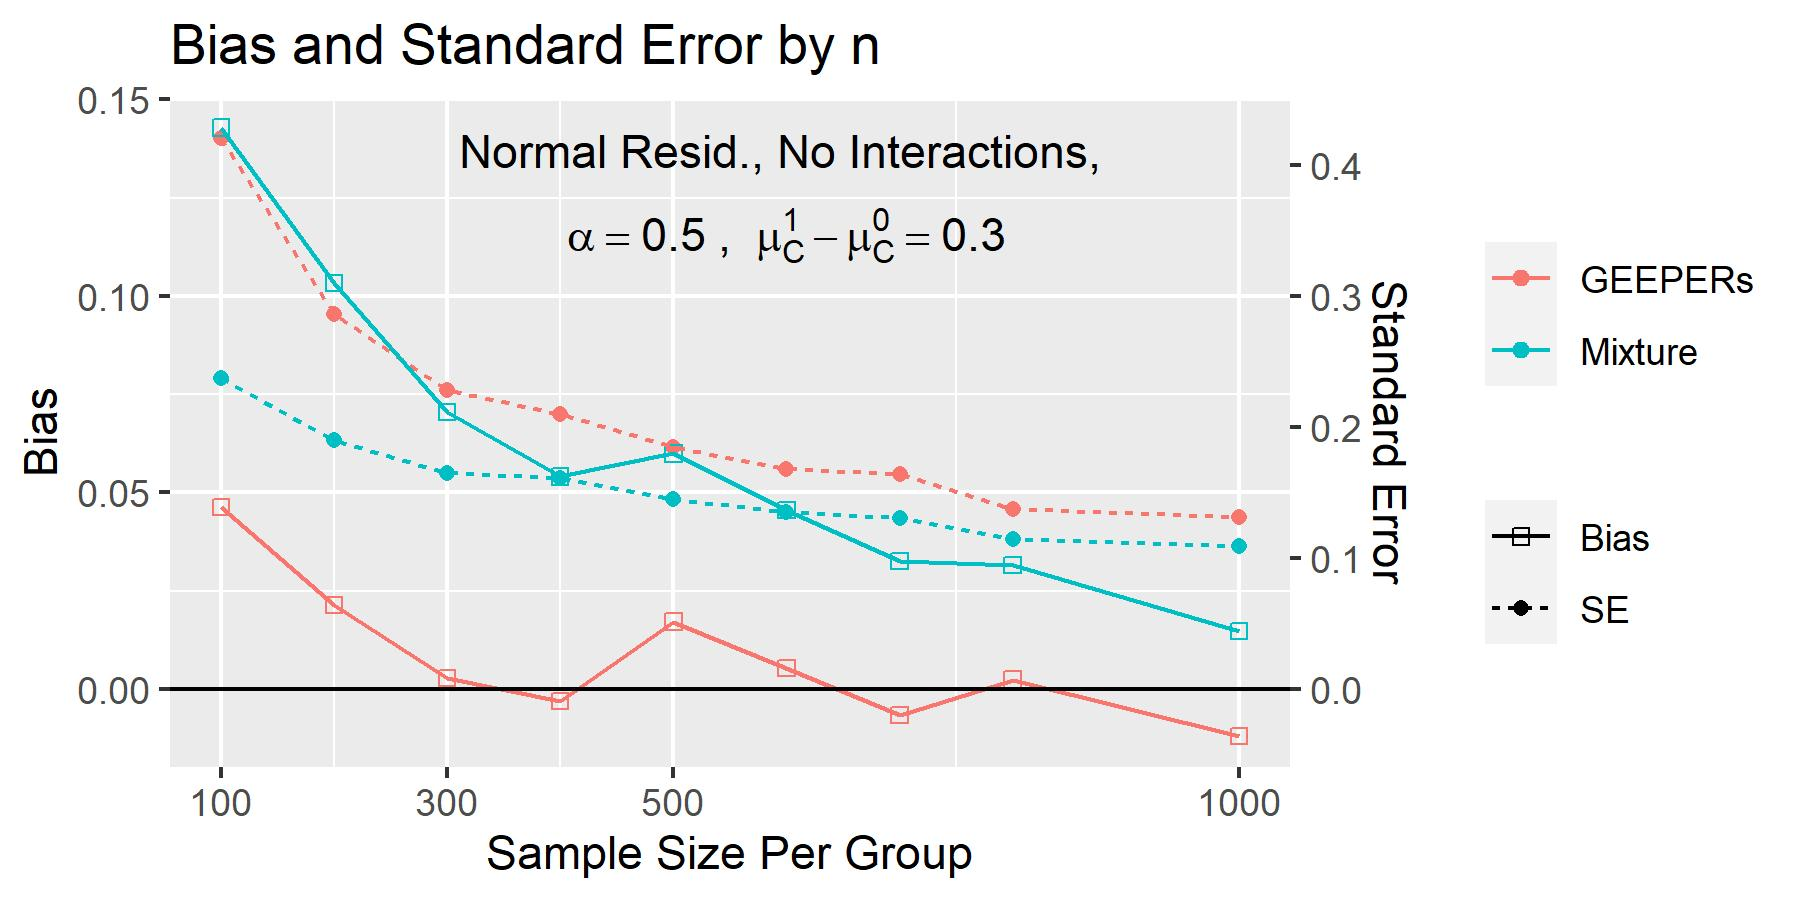
\includegraphics{../simFigs/biasSEbyN.jpg}
  \caption{Empirical bias and standard error of M- and Mixture estimates of $\muc1$ as sample size per treatment group $n$ varies from 0 to 1. There were 500 replications for each $n$. Other factors were held fixed at the noted values.}
  \label{fig:n}
\end{figure}

\begin{figure}
  \centering
  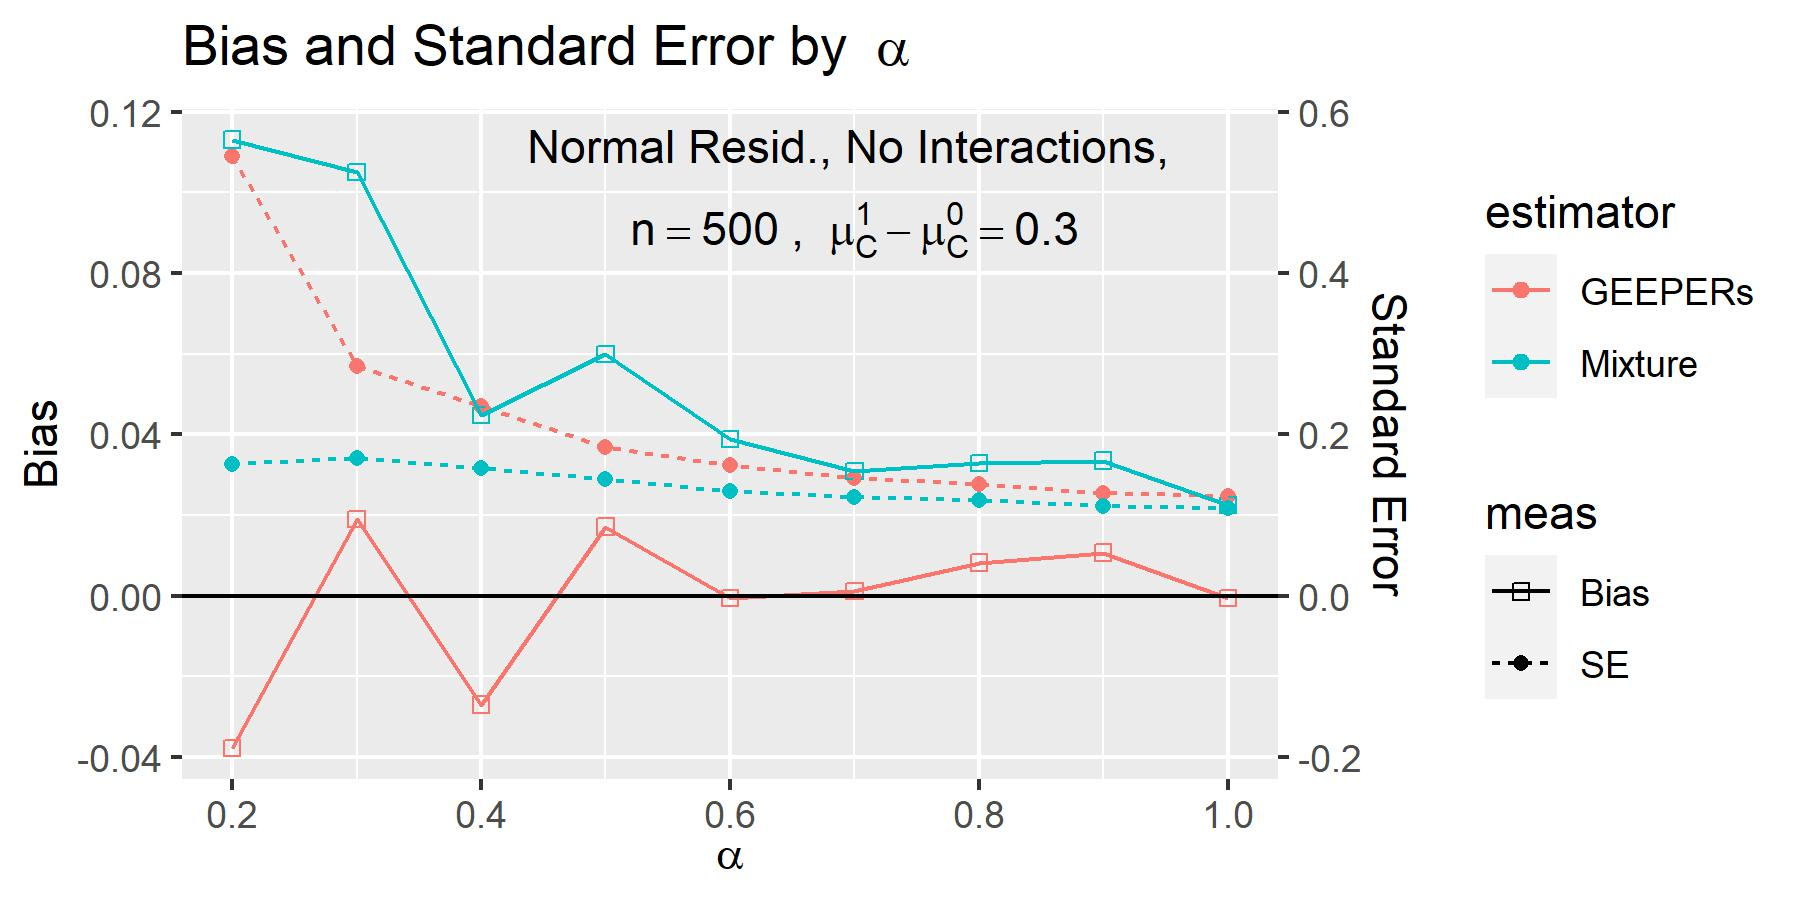
\includegraphics{../simFigs/biasSEbyB1.jpg}
  \caption{Empirical bias and standard error of M- and Mixture estimates of $\muc1$ as $\alpha$ varies from 0.1 to 1. There were 500 replications for each $n$. Other factors were held fixed at the noted values.}
  \label{fig:alpha}
\end{figure}

\subsubsection{Other Factors}


\begin{figure}
  \centering
  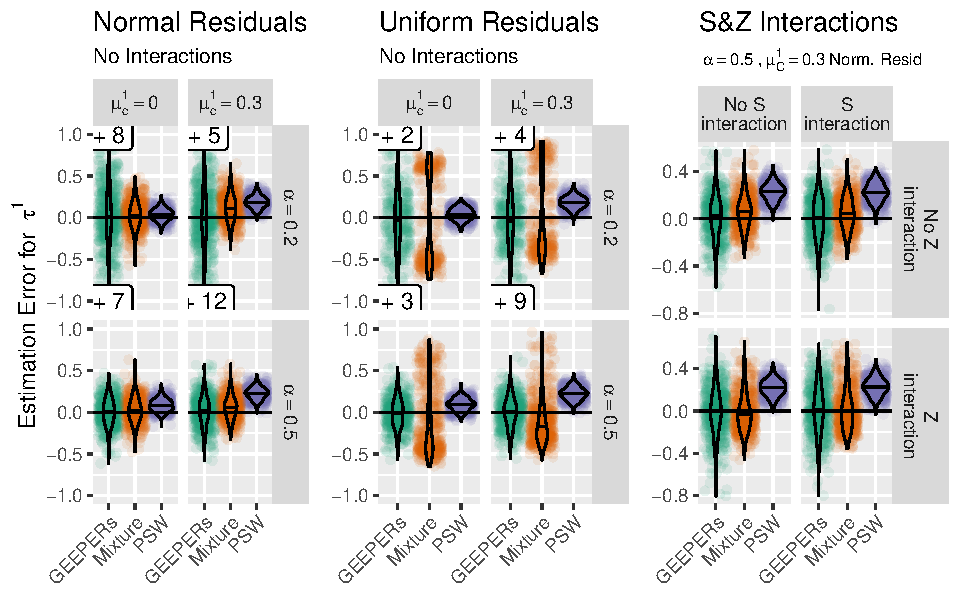
\includegraphics{../simFigs/boxplots.pdf}
  \caption{Violin and scatterplots of 500 simulation estimation errors for estimators described in Section~\ref{sec:simMods} under varying conditions. For all plots, $n=500$; there were 500 replications for each set of conditions. Annotations at the upper and lower edges of the plot indicate the number of extreme outliers excluded from the plotting area.}
  \label{fig:boxplots}
\end{figure}


Figure \ref{fig:boxplots} shows violin plots, layered on top of jitters scatterplots, showing estimation error for the M-estimator, the mixture estimator, and the PSW estimator of $\eff1$ under various sets of conditions, and Table \ref{tab:rmse} shows root mean squared error (RMSE) estimates under a somewhat wider set of circumstances when $\muc1=0.3$.
The leftmost panel of Figure \ref{fig:boxplots} and the top line of Table \ref{tab:rmse} show results under ``standard'' conditions---normal residuals and no interactions in the data generating model between covariates and either $S$ or $Z$.
In this case, the M-estimator is roughly unbiased, but less precise than the other two methods---when $\alpha=0.2$ it is much noisier, and when $\alpha=0.5$ it is only slightly less precise.
The mixture estimator's bias depends on $\muc1$---when $\muc1=0$, the bias is slight, and when $\muc1=0.3$ the bias is more substantial. This is somewhat surprising, because when $\muc1=0$, there is no separation (``dispersion'') between the principal strata in the control group, and previous literature \citep{griffin2008application} has identified this scenario as a particular challenge for mixture modeling.
The PSW estimator is also biased---due, presumeably, to the violation of Principal Ignorability, Assumption \ref{ass:pi}--inherent in the data generating model. On the other hand, the PSW estimator has easily the lowest sampling variance of the three estimators.
In fact, Table \ref{tab:rmse} shows that despite its bias, the PSW estimator has lower RMSE than the M-estimator when $\alpha=0$ or 0.2.
The middle panel of Figure \ref{fig:boxplots} and the fifth line of Table \ref{tab:rmse} shows a similar set of results for when the residuals in \eqref{eq:yc-sim} are uniformly distributed.
In this case, the M-estimator and PSW estimator behave in a similiar fashion to the normal case, but the mixture estimator shows a bimodal pattern--sometimes over-estimating $\eff0$ and sometimes underestimating, but rarely estimationg $\eff1$ accurately.

The rightmost panel of Figure \ref{fig:boxplots} returns to the case of normal residuals---and only shows results when $\muc1=0.3$ and $\alpha=0.5$---but introduces interactions in the data generating model between covariates and either $\st$, $Z$, or both. That is, the coefficients on the covariates in the outcome model vary between principal strata and/or between treatment groups.
Corresponding RMSE results, along with analogous results for uniform residuals and other values for $\alpha$, are in Table \ref{tab:rmse}.
Presence of interactions could undermine the M-estimate by inducing a relationship between principal scores and potential outcomes, even after adjusting the outcomes for covariate effects.
Fortunately, the presence of interactions in the data generating model in this scenario appear to make little difference, though RMSEs were slightly higher when interactions between $Z$ and covariates are present.
Table \ref{tab:rmse} shows that when $\alpha=.2$, M-estimation RMSE can be substantially higher when $Z$ interactions are present than when they are not; plots in the online appendix suggest that this is due to an increase in sampling variance and kurtosis rather than bias.

Table \ref{tab:coverate} shows estimates of the empirical coverage of nominal 95\% confidence intervals for the M-estimator and mixture estimator of $\eff1$, to evaluate their respective standard error estimates and the associated statistical inference.
When $\alpha=0.5$, M-estimator confidence intervals consistently acheive their nominal levels\footnote{With 500 replications and true coverage probabilities of 0.95, the standard error for emperical coverage rates is approximately 1 percentage point.}, whereas confidence intervals from mixture estimators undercover in the presence of interactions between $Z$ and $X$, or when residuals are non-normal.
When $\alpha=0$ or 0.2, M-estimation confidence intervals undercover in the presence of interactions between $X$ and $Z$.
Across all conditions in the table, the M-estimation confidence intervals have higher empirical coverage than their mixture-model counterparts.


%% \begin{figure}
%%   \centring
%%   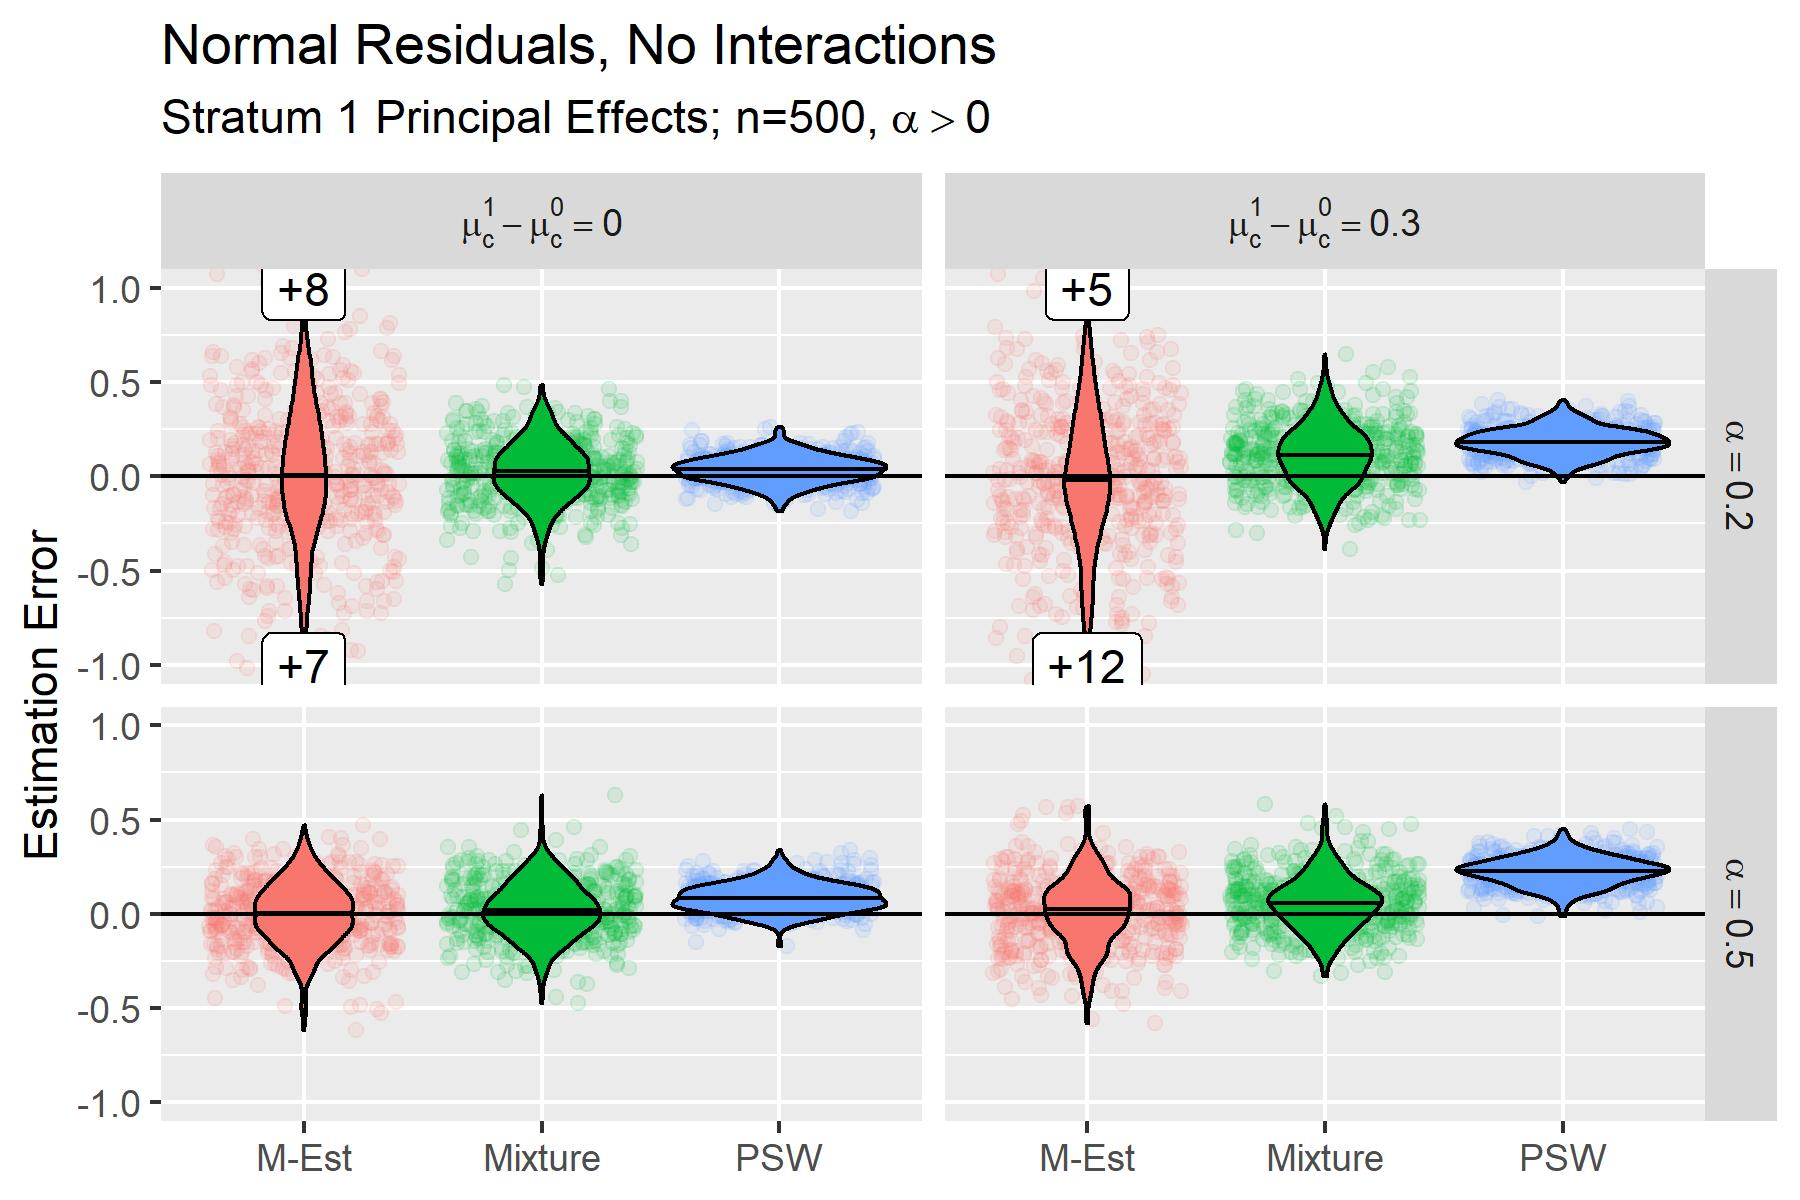
\includegraphics{../simFigs/normalOutcomesNoInteractionPosB1.jpg}
%%   \caption{Violin and scatterplots of 500 simulation estimation errors for estimators described in Section~\ref{sec:simMods} when the distribution of residuals in \eqref{eq:yc-sim} was normal, there were no interactions between covariates and $S$ or $Z$, and $\alpha=0.2,0.5$. Annotations at the upper and lower edges of the plot indicate the number of extreme outliers excluded from the plotting area.}
%%   \label{fig:simNorm}
%% \end{figure}

%% \begin{figure}
%%   \centring
%%   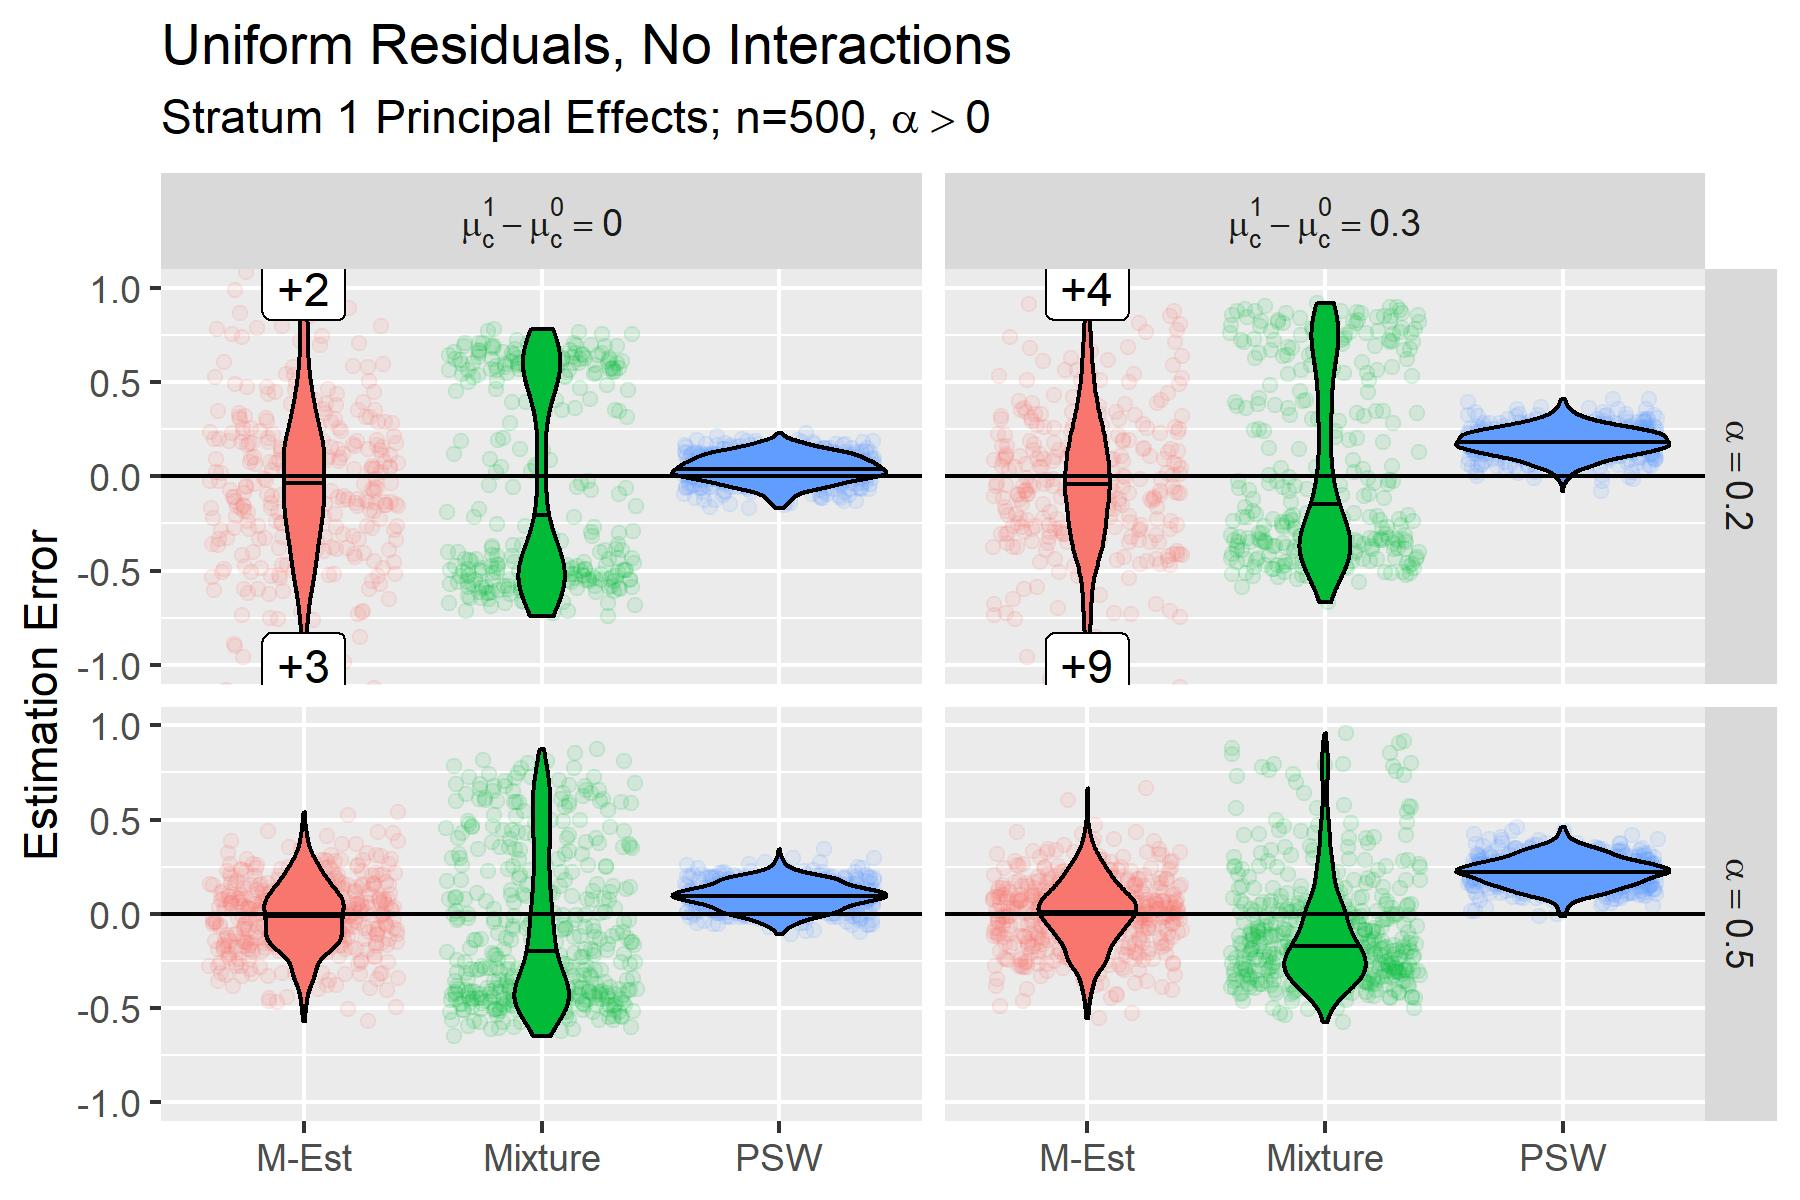
\includegraphics{../simFigs/unifOutcomesNoInteractionPosB1.jpg}
%%   \caption{Violin and scatterplots of 500 simulation estimation errors for estimators described in Section~\ref{sec:simMods} when the distribution of residuals in \eqref{eq:yc-sim} was uniform, there were no interactions between covariates and $S$ or $Z$, and $\alpha=0.2,0.5$. Annotations at the upper and lower edges of the plot indicate the number of extreme outliers excluded from the plotting area.}
%%   \label{fig:simUnif}
%% \end{figure}

%% \begin{figure}
%%   \centring
%%   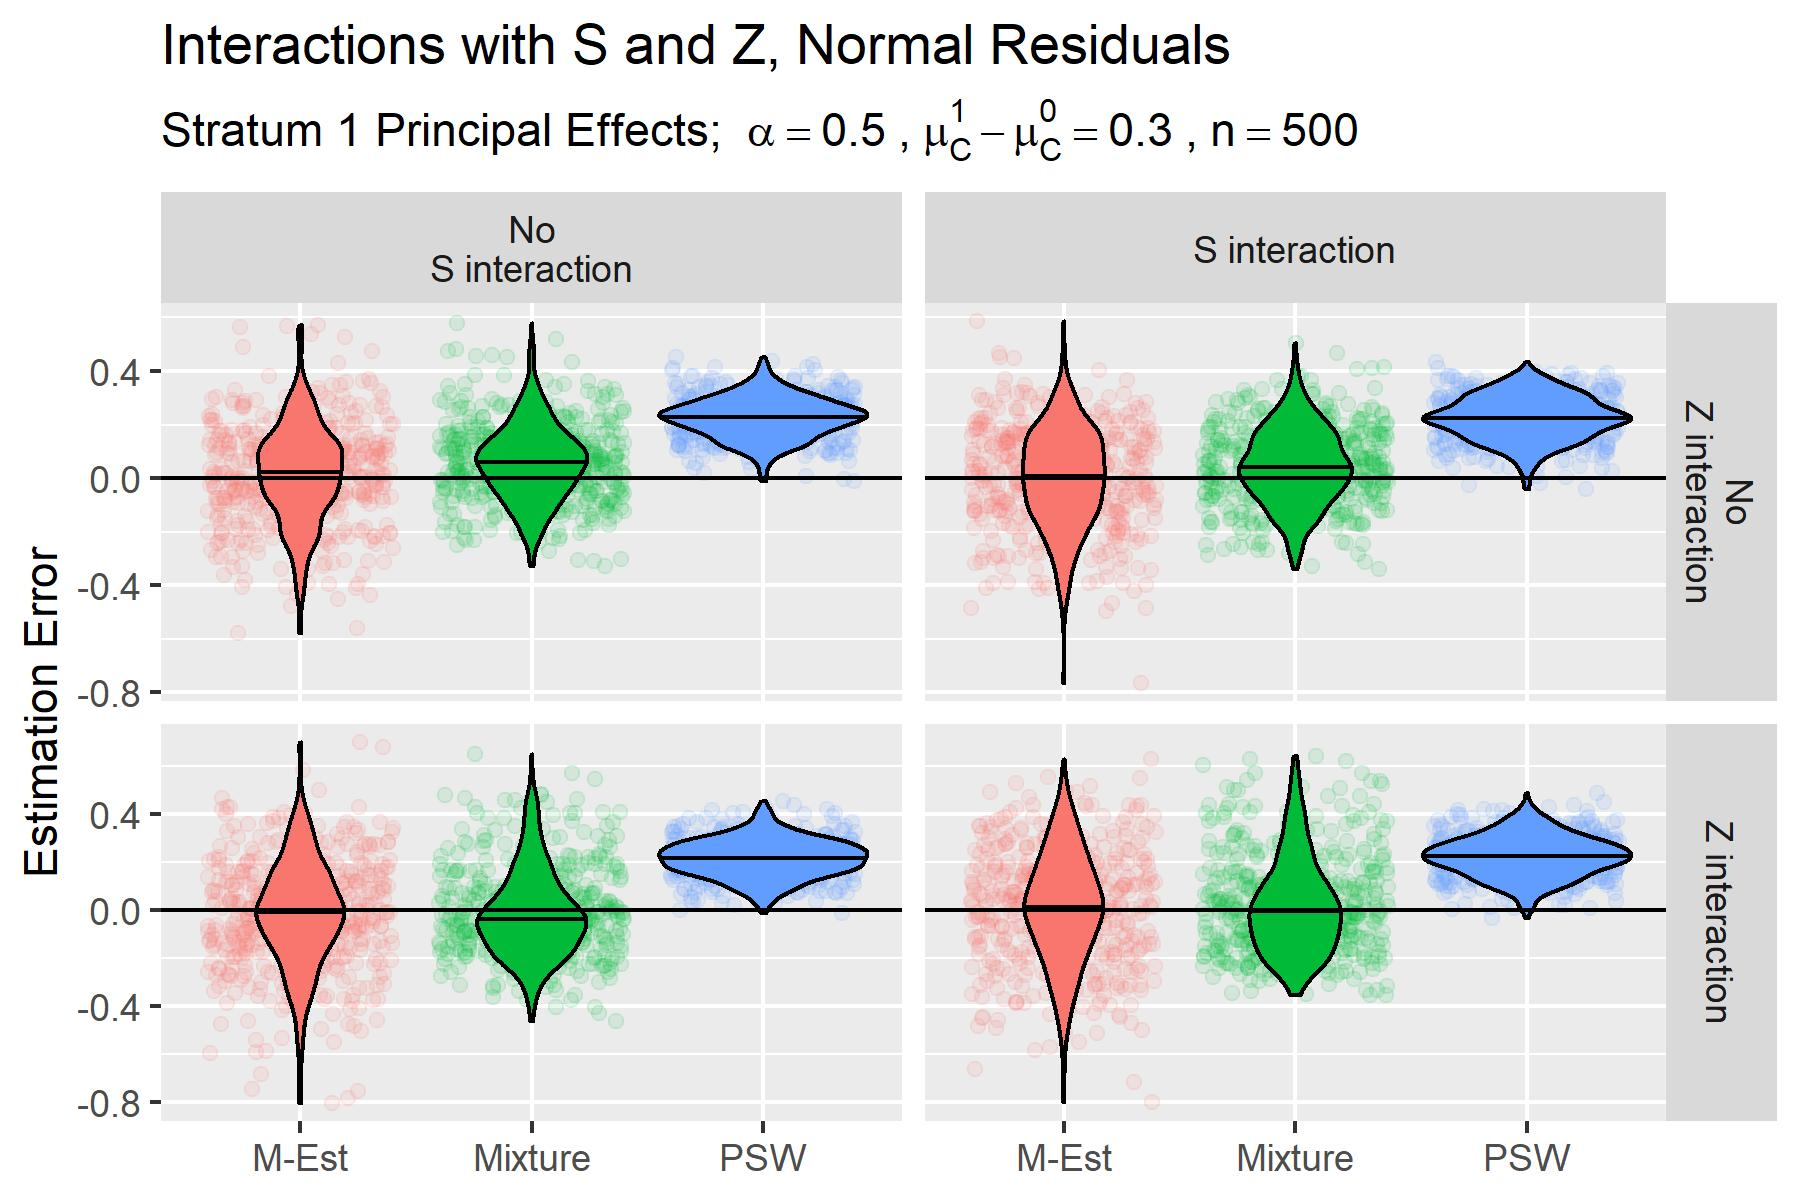
\includegraphics{../simFigs/InteractionPosB1.jpg}
%%   \caption{Violin and scatterplots of 500 simulation estimation errors for estimators described in Section~\ref{sec:simMods} when the distribution of residuals in \eqref{eq:yc-sim} was normal, there were possibly interactions between covariates and $S$ or $Z$, $\muc1=0.3$, and $\alpha=0.5$. Annotations at the upper and lower edges of the plot indicate the number of extreme outliers excluded from the plotting area.}ana
%%   \label{fig:simUnif}
%% \end{figure}


  \begin{table}
    \centering
  
\begin{tabular}[t]{lllrrrrrrrrr}
\toprule
\multicolumn{3}{c}{ } & \multicolumn{3}{c}{$\alpha=0$} & \multicolumn{3}{c}{$\alpha=0.2$} & \multicolumn{3}{c}{$\alpha=0.5$} \\
\cmidrule(l{3pt}r{3pt}){4-6} \cmidrule(l{3pt}r{3pt}){7-9} \cmidrule(l{3pt}r{3pt}){10-12}
\makecell[l]{Residual\\Dist.} & \makecell[c]{X:Z\\Int.?} & \makecell[r]{X:S\\Int.?} & \rotatebox[origin=c]{300}{GEEPERs} & \rotatebox[origin=c]{300}{Mixture} & \rotatebox[origin=c]{300}{PSW} & \rotatebox[origin=c]{300}{GEEPERs} & \rotatebox[origin=c]{300}{Mixture} & \rotatebox[origin=c]{300}{PSW}&\rotatebox[origin=c]{300}{GEEPERs} & \rotatebox[origin=c]{300}{Mixture} & \rotatebox[origin=c]{300}{PSW}\\
\midrule
 & No & No & 2.07 & 0.19 & 0.17 & 0.55 & 0.20 & 0.20 & 0.19 & 0.16 & 0.24\\

 & Yes & No & 9.34 & 0.34 & 0.16 & 1.06 & 0.33 & 0.21 & 0.23 & 0.18 & 0.23\\

 & No & Yes & 2.56 & 0.19 & 0.16 & 0.51 & 0.22 & 0.21 & 0.19 & 0.15 & 0.24\\

\multirow{-4}{*}{\raggedright\arraybackslash Normal} & Yes & Yes & 7.16 & 0.34 & 0.17 & 1.81 & 0.33 & 0.20 & 0.23 & 0.20 & 0.24\\
\cmidrule{1-12}
 & No & No & 4.19 & 0.56 & 0.16 & 0.60 & 0.50 & 0.20 & 0.18 & 0.31 & 0.24\\

 & Yes & No & 6.99 & 0.60 & 0.17 & 0.91 & 0.57 & 0.20 & 0.22 & 0.35 & 0.24\\

 & No & Yes & 1.83 & 0.52 & 0.17 & 0.45 & 0.46 & 0.20 & 0.19 & 0.31 & 0.23\\

\multirow{-4}{*}{\raggedright\arraybackslash Uniform} & Yes & Yes & 7.55 & 0.60 & 0.18 & 1.28 & 0.56 & 0.20 & 0.24 & 0.35 & 0.24\\
\bottomrule
\end{tabular}

  \caption{RMSE }
\end{table}

\begin{table}
  \begin{tabular}[t]{lllrrrrrr}
\toprule
\multicolumn{3}{c}{ } & \multicolumn{2}{c}{$\alpha=0$} & \multicolumn{2}{c}{$\alpha=0.2$} & \multicolumn{2}{c}{$\alpha=0.5$} \\
\cmidrule(l{3pt}r{3pt}){4-5} \cmidrule(l{3pt}r{3pt}){6-7} \cmidrule(l{3pt}r{3pt}){8-9}
\makecell[l]{Residual\\Dist.} & \makecell[c]{X:Z\\Int.?} & \makecell[r]{X:S\\Int.?} & GEEPERs & Mix.  & GEEPERs & Mix. & GEEPERs & Mix.\\
\midrule
 & No & No & 0.99 & 0.99  & 0.97 & 0.97 & 0.96 & 0.96\\

 & Yes & No & 0.88 & 0.74  & 0.88 & 0.74 & 0.94 & 0.89\\

 & No & Yes & 1.00 & 1.00  & 0.98 & 0.97 & 0.97 & 0.96\\
\multirow{-4}{*}{\raggedright\arraybackslash Normal} & Yes & Yes & 0.90 & 0.77  & 0.90 & 0.77 & 0.94 & 0.88\\
\cmidrule{1-9}
 & No & No & 0.99 & 0.29  & 0.97 & 0.40 & 0.95 & 0.61\\

 & Yes & No & 0.83 & 0.11  & 0.87 & 0.20 & 0.93 & 0.48\\

 & No & Yes & 1.00 & 0.47  & 0.98 & 0.53 & 0.96 & 0.57\\

\multirow{-4}{*}{\raggedright\arraybackslash Uniform} & Yes & Yes & 0.83 & 0.15 & 0.88 & 0.21 & 0.94 & 0.53\\
\bottomrule

\end{tabular}

  \caption{Coverage}
  \label{tab:coverage}
\end{table}


\section{Application: Estimating Treatment Effects for Implementation Subgroups}

In a recent educational field experiment, middle school students completing their math schoolwork on a computer program were randomized between four conditions. In all four conditions, students worked on their assigned math program in class on 12 different occassions---a prior assessmenent, a mid-test, a post-test, and nine learning sessions---spaced throughout the school year.  In three of the conditions, during the learning sessions, students worked through a series of math problems, while the forth condition was a computer game designed to teach math concepts. In this illustration, we will consider three different treatment effects, comparing one of the four conditions (which we arbitrarily label ``treatment''), with each of the three others (Business as Usual, or ``BAU'', From-Here-To-There!, or ``FH2T,'' and DragonBox), separately. During learning sessions, students in the treatment condition received immediate, informative error messages after entering a wrong answer, and were required to enter a correct answer in order to proceed. They also had access to a series of hints for each problem, the last of which (called the ``bottom out'' hint) contained the correct answer. Students in the other three conditions did not have access bottom out hints; our illustration will focus on that software feature.

The literature on hints in online learning is mixed \citep{stuff}, in particular when it comes to requesting a bottom-out hint (called ``bottoming out''). On the one hand, hints that include the correct answer are essentially worked examples, which can be beneficial to learning \citep{worked example stuff}. On the other hand, they allow students to ``game the system,'' by simply requesting enough hints to see the right answer, and use the software without ever working to solve any problems. However, in this experiment, the ability to bottom out was only one of several differnces between the treatment conditions. One way to disentangle the role of bottoming out in any treatment effect would be to estimate average treatment effects separately for subjects who would (if assigned to treatment) bottom out, and for subjects who would not. If hints (that do not supply the correct answer) and error messages are helpful, but the ability to bottom out is harmful to learning, then we might expect to estimate a positive effect of being assigned to the feedback condition for students who do not bottom out, but a negative effect for students who do. If hints are helpful for learning only if they can be read as worked examples, then we might expect no effect of condition on students who do not bottom out, but a positive effect for students who do. (These hypothetical results may be masked by other treatment effect heterogeneity between students who would or wouldn't bottom out, but the results could still be informative.)

For the purpose of demonstrating GEEPERS, we gathered dichotomized data on %which students in the treatment condition requested at least one bottom-out hint.
whether students in the treatment condition requested more than the median number of bottom-out hints (11).
That is, $\st=1$ for students who, if assigned to the treatment condition, would request at more than 11 bottom-out hints (``bottom-outers''), and $\st=0$ for students who would request 11 or fewer (``non-bottom-outers''). %least one bottom-out hint, and $\st=0$ for students who would not.
The outcome of interest $Y$ in our example is students' total scores on a ten-item posttest completed within the online tutoring system; $Y$ is an integer ranging from 0 to 10.
The goal of our analysis will be to determine the principal effects $\tau_1=\EE[\yt-\yc|\st=0]$ and $\tau_0=\EE[\yt-\yc|\st=0]$, the average effects of assignment to the treatment condition for bottom-outers and non-bottom-outers.

We also had access to data on a number of baseline covariates: total scores on a 10-item pretest, fifth-grade stanardized test scores, race/ethnicity (white, Asian, Hispanic/Latino, or Other), indicator variables for if students have an early intervention program (EIP) or individualized educational plan (IEP) in place, if students are learning English as a second language (ESOL), students' average time on task for the pretest (logged), total scores from baseline evaluations of students' math anxiety, negative reaction to math, and numerical confidence, and an indicator for weather students began the school year in remote or in-person instruction.
Students with missing pretest scores were dropped from the analysis; missing data in other covariates was imputed with a Random Forest algorithm \citep{missForest}.
Table \ref{tab:tab1} describes each covariate--as well as the sucess of the randomForest imputation algorithm.

\begin{table}
  \centering
  \small
\begin{tabular}[t]{llllll}
\toprule
  & level & ASSISTments & BAU & Miss. \% & Imp. Err.\\
\midrule
\addlinespace[0.3em]
\multicolumn{6}{l}{\textbf{Baseline}}\\
n &  & 461 & 428 &  & \\
Pretest &  & -0.22 (2.63) & -0.37 (2.64) & 0.0 & 0\\
Gr. 5 Stand. Test &  & 578.16 (60.39) & 580.87 (59.71) & 11.5 & 1754.93\\
Gender  (n (\%)) & Female & 202 (49.3) & 176 (46.2) & 11.0 & \\
 & Male & 208 (50.7) & 205 (53.8) &  & \\
Race/Eth. (n (\%)) & White & 100 (44.2) & 73 (36.3) & 52.0 & \\
 & Asian & 40 (17.7) & 44 (21.9) &  & \\
 & Hispanic & 42 (18.6) & 32 (15.9) &  & \\
 & Other & 44 (19.5) & 52 (25.9) &  & \\
Has EIP (n (\%)) &  & 27 ( 6.6) & 28 ( 7.4) & 11.5 & 0.08\\
Has IEP (n (\%)) &  & 39 ( 9.5) & 33 ( 8.7) & 11.0 & 0.1\\
ESOL (n (\%)) &  & 23 ( 5.6) & 33 ( 8.7) & 11.0 & 0.04\\
Gifted (n (\%)) &  & 71 (17.3) & 73 (19.2) & 11.0 & 0.16\\
log(Pretest ToT) &  & 4.14 (0.71) & 4.16 (0.81) & 0.0 & 0\\
Math Anxiety &  & 13.35 (5.77) & 13.50 (5.70) & 6.0 & 0.31\\
Math Neg. React. &  & 3.06 (2.31) & 3.13 (2.33) & 6.0 & 1.29\\
Numerical Conf. &  & 4.75 (2.67) & 4.81 (2.70) & 6.0 & 2.07\\
\addlinespace[0.3em]
\multicolumn{6}{l}{\textbf{Post-Treatment}}\\
Posttest &  & 4.44 (2.84) & 4.37 (2.87) & 32.6 & \\
Bottom Out (\%) &  & 222 (48.2) & 0 ( 0.0) & 0.0 & \\
\bottomrule
\end{tabular}

  \caption{Descriptive statistics on baseline covariates, $S$, and $Y$ for the analysis data. Values are mean (SD) unless otherwise noted. Imputation error is the ``out of box'' error estimate from the Random Forest imputation algorithm---root mean squared error divided by the observed standard deviation for continuous variables and misclassification proportion for categorical variables.}
  \label{tab:tab1}
\end{table}

The data analysis we present here is intended as a demonstration of GEEPERS, rather than for its substantive conclusions, and our description omits discussion of some important methodological considerations, including attrition and post-selection inference. For a more complete discussion of the experimental design, the conditions being compared, and the impact analysis, please see \citet{impactPaper}.

\subsection{Principal Score Model}

\begin{figure}
  \centering
  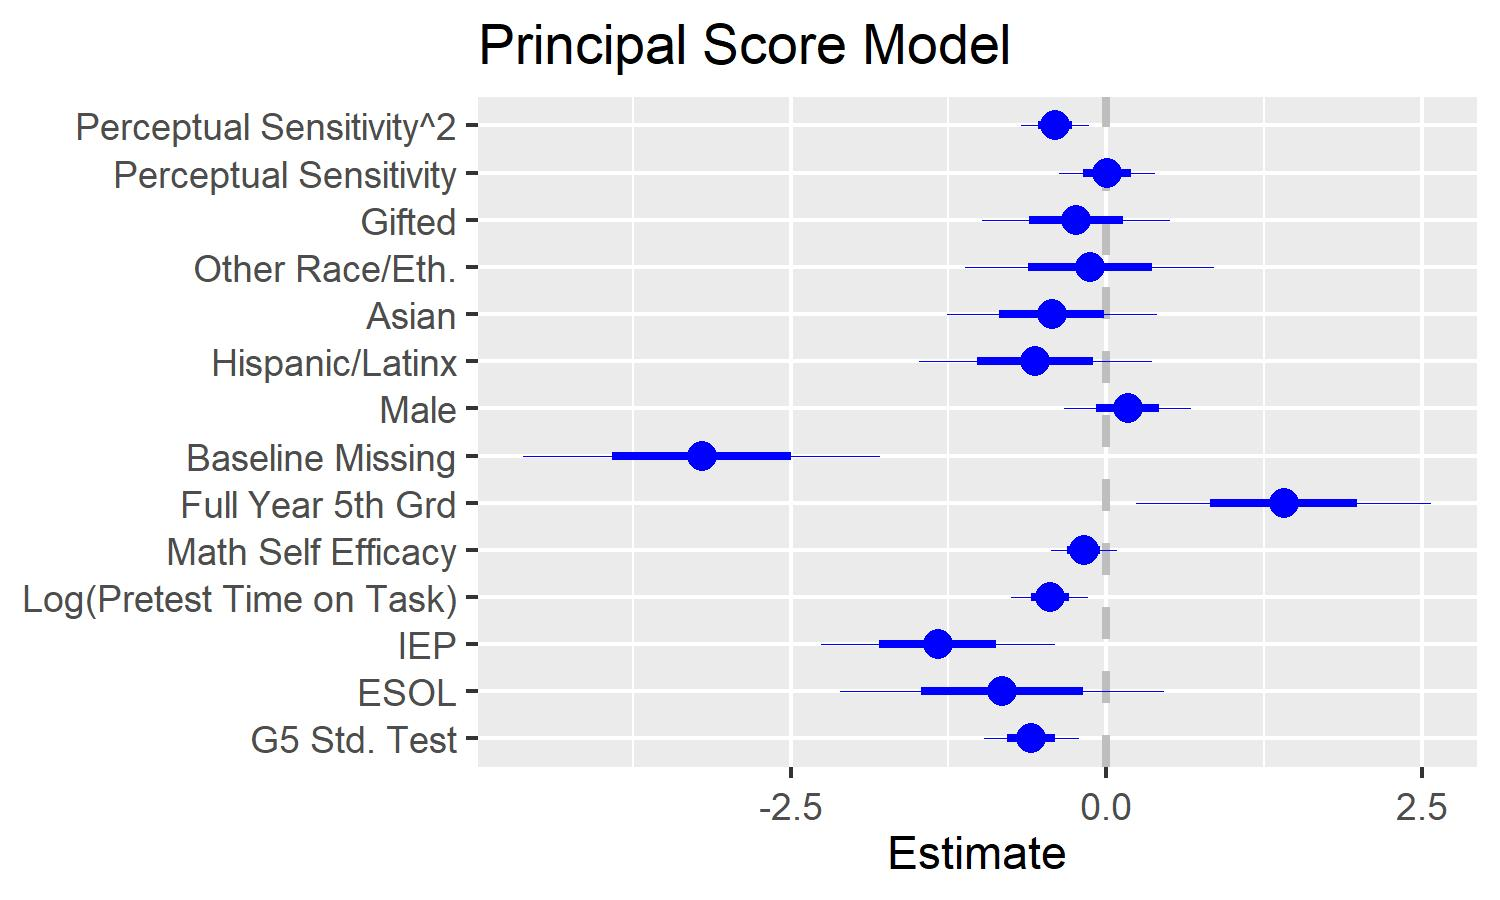
\includegraphics{../figure/psModCoef.jpg}
  \caption{Principal Score Model Coefficients}
  \label{fig:psMod}
\end{figure}


We considered several models for the principal score, and full results (which are largely similar to each other) can be found in the online appendix. Here we present results from our model of choice, a logistic regression of observed $S$ on baseline variables chosen with a combination of expert judgement and backwards selection based on the AIC. These included school fixed effects and a set of student-level demographic and educational data: fifth-grade mathematics standardized test scores, %Gender, Race/Ethnicity,
indicator variables for special education status (IEP), whether the student was taking English as a second language (ESOL), whether the student was classified as gifted, and whether students attended a full year of school in 5th grade. Finally, we also included data collected from students at the beginning of the study: the natural logrithm of the  time spent on task during the pretest, scores on baseline measurements of mathematics anxiety and self-efficacy and perceputal sensitivity, along with a missingness indicator for these measurements.
Binned residual plots \citep{gelman2006data} from an initial model fit indicated a curviliniar relationship between percentual sensitivity measurements (modeled as linear) and model errors, so in the final model we included perceptual sensitivity as a quadratic polynomial.
The model was fit to data from students in the treatment group, for whom bottom-out status ($S$) was observed; hence, the same model fit was used for all three treatment contrasts.

The model was fairly successful in distinguishing bottom-outers from non-bottom-outers---the AUC, evaluated using out-of-sample predictions in a 10-fold cross-validation, was roughly 0.795. That is, in roughly 80\% of bottom-outer/non-bottom-outer pairs of subjects, the bottom-outer will have a higher predicted probability from the model.
Table \ref{tab:results} show the model's coefficient estimates. Noteably, conditional on the other covariates, students with higher fifth-grade standardized test scores were less likely to request many bottom out hints, as were students who spent little time on task during the pretest, while IEP and ESOL students, and students without baseline measurement data, were relatively unlikely to be bottom-outers. The relationship between perceptual sensitivity and bottom out requests was not monotonic---students with average levels were more likely than those with more extreme high or low levels to be bottom-outers; bottom-outers tended to have lower math self-efficacy, but the data are also consistent with a small positive relationship, and there appears to be little to no relationship between math anxiety and bottom-outer status at all.


\subsection{Outcome Regression and Principal Effects}
\begin{figure}
  \centering
  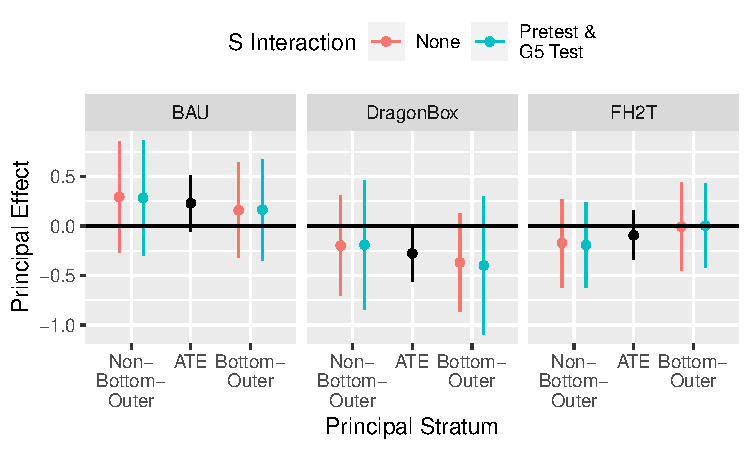
\includegraphics{../figure/prinEffs.pdf}
  \caption{Principal Effects}
  \label{fig:effects}
\end{figure}

Figure \ref{fig:effects} plots the estimated principal effects for bottom-outers and non-bottom-outers, using two different models---alongside estimates of the overall average treatment effect, labeled ``ATE.'' In both models, effects were adjusted for all of the variables that were in the principal score model, in addition to students' pretest scores; also, the models substituted class fixed effects for school fixed effects.\footnote{Why use a corser set of fixed effects for the principal score model than the outcome regression? There were two reasons: first, the principal score model was fit to a smaller sample (only students in the ``Instant'' condition), so some classrooms only included one student, which can lead to poor fit. Second, the asymptotics of logistic regression are more restricted than OLS, and so logistic regression tends to perform poorly when the number of parameters increases with the sample size \citep{agresti}.}
The two sets of esimated differed in that the first assumed that coefficients on covariates were equal across principal strata, whereas the second set of results allowed the coefficients on pretest and 5th-grade standardized test scores---the most important predictors of outcomes and principal strata membership, respectively---to vary between strata.

The results suggest little difference, if any, between the effects in the two principal strata.
Estimated effects compared to BAU or DragonBox were slightly lower for bottom-outers than for non-bottom-outers, and estimated effects compared to FH2T were higher for non-bottom-outers.
However, none of these differences is statistically significant, so opposite patterns, or no difference betweeen principal effects at all, would also be consistant with the data.
In fact, 95\% confidence intervals for all principal effects include both positive and negative principal effects.
There is no discernable difference between estimated principal effects when coefficients on pretest and grade-5 standardized tests were or were not allowed to vary between strata, though standard errors from the models including an interaction were somewhat higher.

\subsection{Mixture Model and Principal Score Weighting}
\begin{figure}
  \centering
  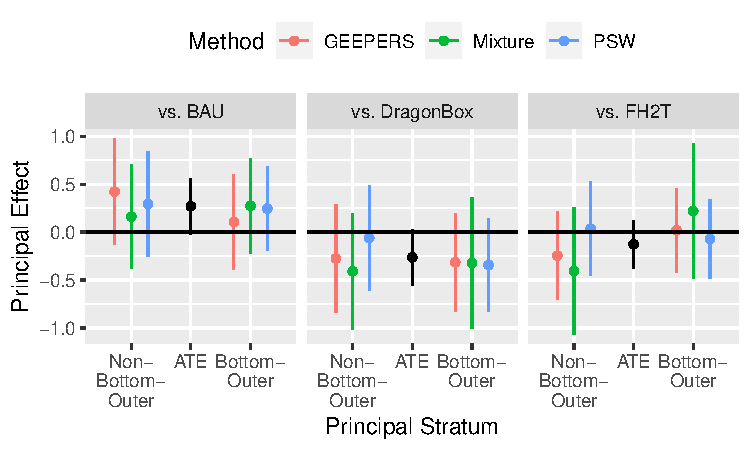
\includegraphics{../figure/compareMethods.pdf}
  \caption{Principal Effects}
  \label{fig:compare}
\end{figure}



\section{Discussion}

\appendix
\section{Proofs and Calculations}
\subsection{Proof for Lemma \ref{lemma:expectation}}
As a preliminary, note that
% \begin{align*}
%   \EE[\st|\hpp]&=\EE\left\{\EE[\st|\pp,\hpp]|\hpp\right\}\\
%              &=\EE\left\{\EE[\st|\pp]|\hpp\right\}\\
%              &=\EE[\pp|\hpp]=\hpp
% \end{align*}

%Then, note
\begin{align*}
  \EE[Y_C|\pp]&=\EE\left\{\EE[Y_C|\pp,\st]|\pp\right\}\\
             &=\EE\left\{\EE[Y_C|\st]|\pp\right\}\tag*{by \eqref{eq:assumption}}\\
             &=\EE[\muc1\st+\muc0(1-\st)|\pp]\\
             &=\muc1\pp+\muc0(1-\pp)
\end{align*}

Then we have
\begin{equation*}
  \begin{split}
    \EE[Y_C]=&\EE\EE[Y_C|\pp]=\muc1\EE\pp+\muc0(1-\EE\pp)\\
    =&\muc0+\EE\pp(\muc1-\muc0)
    \end{split}
\end{equation*}

Next we have

\begin{align*}
  \EE[Y_C\pp]&=\EE\left\{\EE[Y_C\pp|\pp]\right\}\\
            &=\EE\left\{\pp\EE[Y_C|\pp]\right\}\\
            &=\EE\left\{\pp\left[\muc1\pp+\muc0(1-\pp)\right]\right\}\\
            &=\EE[\pp]\muc0+\EE[\pp^2](\muc1-\muc0)
\end{align*}

In the treatment group, $\st$ is observed, so
\begin{align*}
    \EE[Y_T]=&\mut0+\EE[\st](\mut1-\mut0)\tag*{and}\\
    \EE[\st Y_T]=&\EE[\st]\mut0+\EE[\st^2](\mut1-\mut0)
\end{align*}

Due to Assumption \ref{ass:rand} (randomization), $\EE[Y|Z=0]=\EE[Y_C]$, $\EE[Y|Z=1]=\EE[Y_T]$, $\EE[Y\pp|Z=0]=\EE[Y_C\pp]$ and $\EE[YS|Z=1]=\EE[Y_T\st]$, completing the proof.

\subsection{Proof for Proposition \ref{prop:reg0}}
Carrying out those replacements in \eqref{eq:estEq0}, and rearranging\footnote{Technically, replacing $\tilde{\Psi}_i$ with $\Psi_i=\begin{psmallmatrix} 1 & 0&1&0\\ 0&1&0&1\\0&0&1&0\\0&0&0&1\end{psmallmatrix}\tilde{\Psi}_i$.} gives an equivalent set of estimating equations:
\begin{equation}\label{eq:estEq1}
\sum_{i=1}^{n_C}\Psi_i=\sum_{i=1}^{n_C}\begin{pmatrix}
    Y_i-\muc0-\ri(\muc1-\muc0)-Z_i(\mut0-\muc0)-Z_i\ri(\mut1-\mut0-\muc1+\muc0)\\
    \ri Y_i-\ri\muc0-\ri^2(\muc1-\muc0)-Z_i\ri(\mut0-\muc0)-Z_i\ri^2(\mut0-\mut1-\muc0+\muc1)\\
    Z_iY_i-Z_i\mut0-Z_i\ri (\mut1-\mut0)\\
    Z_i\ri Y_i -Z_i\ri\mut0-Z_i\ri^2(\mut1-\mut0)

\end{pmatrix}=\begin{pmatrix} 0\\0\\0\\0\end{pmatrix}
\end{equation}

\subsection{Proof for Proposition \ref{prop:interaction}}
First, note that $\EE[S]=\EE\EE[S|\bx]=\EE[\pp]$ and
$$\EE[\bx S]=\EE[\bx S|Z=1]=\EE[\bx S|Z=0]=\EE[\bx \EE[\bx\EE[S|\bx]|Z=0]]=\EE[\bx\pp|Z=0]=\EE[\bx\pp]$$
implying that
\begin{equation*}
  \begin{split}
    \EE[Y|\bx,Z=0]&=\beta_0+\bm{\beta_1}\bxy+\beta_2\pp+\bm{\beta_5}'\bxy\pp\\
    \EE[Y|\bx,S,Z=1]&=\beta_0+\beta_3+(\bm{\beta_1}+\bm{\beta_6})\bxy+(\beta_3+\beta_4)S+(\bm{\beta_5}+\bm{\beta_7})'\bxy S
  \end{split}
\end{equation*}
Therefore,
\begin{align*}
  \EE[Y]&=\EE[Y|Z=0]+\EE[Z]\left\{\EE[Y|Z=1]-\EE[Y|Z=0]\right\}\\
  &=\beta_0+\bm{\beta_1}\EE[\bxy]+\beta_2\EE[\pp]+\bm{\beta_5}'\EE[\bxy\pp]+\EE[Z]\left\{\beta_3+\bm{\beta_4}\EE[S]+\bm{\beta_6}'\EE[\bxy]+\bm{\beta_7}'\EE[\bxy S]\right\}\\
  &=\beta_0+\bm{\beta_1}\EE[\bxy]+\beta_2\EE[R]+\bm{\beta_5}'\EE[\bxy R]+\EE[Z]\left\{\beta_3+\bm{\beta_4}\EE[R]+\bm{\beta_6}'\EE[\bxy]+\bm{\beta_7}'\EE[\bxy R]\right\}\\
\end{align*}
Analogous reasoning leads to expressions for $\EE[RY]$, $\EE[\bxy Y]$, $\EE[ZY]$,  $\EE[ZRY]$, $\EE[\bxy YZ]$, and $\EE[\bxy RZY]$.
These, in turn, give rise to estimating equations
\begin{equation*}
  \displaystyle\sum_i \begin{pmatrix}
    Y_i-\beta_0-\bm{\beta_1}\bxy_i-\beta_2R_i-\bm{\beta_5}'\bxy_iR_i-Z_i\left\{\beta_3-\bm{\beta_4}R_i-\bm{\beta_6}'\bxy_i-\bm{\beta_7}'\bxy_i R_i\right\}\\
    R_iY_i-\beta_0R_i-\bm{\beta_1}\bxy_i R_i-\beta_2R_i^2-\bm{\beta_5}'\bxy_iR_i^2-Z_i\left\{\beta_3R_i-\bm{\beta_4}R_i^2-\bm{\beta_6}'\bxy_iR_i-\bm{\beta_7}'\bxy_i R_i^2\right\}\\
    \bxy_i Y_i-\beta_0\bxy_i-\bm{\beta_1}\bxy_i\bx^{Y'}_i-\beta_2R_i\bxy_i-\bm{\beta_5}'\bxy_iR_i-Z_i\left\{\beta_3\bxy_i-\bm{\beta_4}R_i\bxy_i-\bm{\beta_6}'\bxy_i\bx^{Y'}_i-\bm{\beta_7}'\bxy_i\bx^{Y'}_i R_i\right\}\\
    Z_iY_i-Z_i\left\{\beta_0-\bm{\beta_1}\bxy_i-\beta_2R_i-\bm{\beta_5}'\bxy_iR_i-\beta_3-\bm{\beta_4}R_i-\bm{\beta_6}'\bxy_i-\bm{\beta_7}'\bxy_i R_i\right\}\\
    Z_iR_iY_i-Z_iR_i\left\{\beta_0-\bm{\beta_1}\bxy_i-\beta_2R_i-\bm{\beta_5}'\bxy_iR_i-\beta_3-\bm{\beta_4}R_i-\bm{\beta_6}'\bxy_i-\bm{\beta_7}'\bxy_i R_i\right\}\\
    Z_iY_i\bxy_i-Z_i\left\{\beta_0\bxy_i-\bm{\beta_1}\bxy_i\bx^{Y'}_i-\beta_2R_i\bxy_i-\bm{\beta_5}'\bxy_i\bx^{Y'}_iR_i-\beta_3\bxy_i-\bm{\beta_4}R_i\bxy_i-\bm{\beta_6}'\bxy_i\bx^{Y'}_i-\bm{\beta_7}'\bxy_i\bx^{Y'}_i R_i\right\}\\
    R_iZ_iY_i\bxy_i-Z_iR_i\left\{\beta_0\bxy_i-\bm{\beta_1}\bxy_i\bx^{Y'}_i-\beta_2R_i\bxy_i-\bm{\beta_5}'\bxy_i\bx^{Y'}_iR_i-\beta_3\bxy_i-\bm{\beta_4}R_i\bxy_i-\bm{\beta_6}'\bxy_i\bx^{Y'}_i-\bm{\beta_7}'\bxy_i\bx^{Y'}_i R_i\right\}
  \end{pmatrix}=\begin{pmatrix} 0\\0\\0\\0\\0\\0\\0\end{pmatrix}
\end{equation*}
These are the estimating equations for the regression model \eqref{eq:fullInteractionModel}, fit by OLS. Now note that
\begin{equation*}
  \EE[Y_T-Y_C|\st=0]=\beta_0^T-\beta_0^C+(\bm{\beta_1}^{T'}-\bm{\beta_1}^{C'})\EE[\bxy|S=0]=\beta_3+\beta_6'E[\bxy|S=0]
\end{equation*}
and
\begin{equation*}
  \EE[Y_T-Y_C|\st=1]=\beta_0^T+\beta_2^T-(\beta_0^C+\beta_2^C)+(\bm{\beta_1}^{T'}+\bm{\beta_3^{Ti}}-\bm{\beta_1}^{C'}-\bm{\beta_3^{C'}})\EE[\bxy|S=0]=\beta_3+\beta_4+(\beta_6'+\beta_7')E[\bxy|S=1]
\end{equation*}
the result follows

\end{document}
